% !TEX TS-program = pdflatex
% !BIB TS-program = bibtex

\documentclass{ccjnl}

\usepackage[T1]{fontenc}
\usepackage{textcomp}
\usepackage{tabularx}
\usepackage{xcolor}
\colorlet{BLUE}{blue}
\newcommand{\rev}[1]{{\color{blue}#1}}
\DeclareUnicodeCharacter{FF0C}{, }
\DeclareUnicodeCharacter{FF1A}{: }
\DeclareUnicodeCharacter{FF08}{(}
\DeclareUnicodeCharacter{FF09}{)}
\DeclareUnicodeCharacter{FF1B}{; }
\DeclareUnicodeCharacter{3002}{. }
\DeclareUnicodeCharacter{FF1F}{? }
\DeclareUnicodeCharacter{FF01}{! }
\usetikzlibrary{shapes.geometric,shapes,arrows.meta,positioning,fit,calc}
\renewcommand{\qedsymbol}{}

\title{System Relaxation for Resilient Network Governance: A Model-Driven Control Mechanism Against Structural Stress Concentration}
\author{Jie Ding\inst{1}, Zhiyuan Ren\inst{2,*}, Yuehan Li\inst{2}, Wenchi Cheng\inst{2}, Zhiliang Shuai\inst{2}\corinfo{zyren@xidian.edu.cn}}
\receiveddate{}
\reviseddate{}
\Editor{}

\address[1]{National Key Laboratory of Multi-domain Data Collaborative Processing and Control, Yard No. 13, Dacheng Road, Fengtai District, Beijing, China}
\address[2]{School of Telecommunications Engineering, Xidian University, Xi'an 710071, China}

\def\publishmonth{5}
\def\publishyear{2026}

\usepackage{booktabs,enumitem}
\AtBeginDocument{%
\setlength{\abovedisplayskip}{5.5pt plus 2pt minus 2pt}%
\setlength{\belowdisplayskip}{5.5pt plus 2pt minus 2pt}%
\setlength{\abovedisplayshortskip}{3pt plus 1pt minus 1pt}%
\setlength{\belowdisplayshortskip}{3pt plus 1pt minus 1pt}%
\setlength{\textfloatsep}{8pt plus 2pt minus 2pt}%
\setlength{\floatsep}{6pt plus 2pt minus 2pt}%
\setlength{\intextsep}{6pt plus 2pt minus 2pt}%
\setlength{\dbltextfloatsep}{8pt plus 2pt minus 2pt}%
\setlength{\dblfloatsep}{6pt plus 2pt minus 2pt}%
}
\setlist[itemize]{leftmargin=1.4em,itemsep=1.5pt,topsep=2.5pt,parsep=0pt}
\setlist[enumerate]{leftmargin=1.6em,itemsep=1.5pt,topsep=2.5pt,parsep=0pt}
\pdfstringdefDisableCommands{%
  \def\rev#1{#1}%
  \def\widetilde#1{#1}%
  \def\kappa{k}%
  \def\alpha{alpha}%
  \def\beta{beta}%
}

\titlespacing*{\section}{0pt}{8pt plus 2pt minus 2pt}{4pt plus 1pt minus 1pt}
\titlespacing*{\subsection}{0pt}{6pt plus 2pt minus 1pt}{3pt plus 1pt minus 1pt}
\titlespacing*{\subsubsection}{0pt}{4pt plus 1pt minus 1pt}{2pt plus 1pt minus 1pt}
\renewcommand{\topfraction}{0.92}
\renewcommand{\bottomfraction}{0.85}
\renewcommand{\textfraction}{0.08}
\renewcommand{\floatpagefraction}{0.85}
\renewcommand{\dbltopfraction}{0.92}
\renewcommand{\dblfloatpagefraction}{0.85}
\begin{document}
\maketitle

\begin{abstract}
Prevailing network control strategies, rooted in static shortest-path logic, inherently suffer from ``stress concentration,'' where traffic excessively gravitates toward critical nodes, causing structural vulnerabilities and premature capacity saturation. \rev{Existing dynamic link-weight optimization, reactive queue-aware routing, and AI-driven methods either operate in an open-loop manner, oscillate under delayed feedback due to the absence of temporal state damping, or lack formal stability guarantees.} To address this, we introduce the System Relaxation Algorithm (SRA), a model-driven supervisory governance layer inspired by physical relaxation that guides the network toward a ``relaxed'' emergent equilibrium of load balance. SRA functions as an interpretable ``white-box'' dynamical system where node costs evolve based on historically accumulated structural stress \rev{generalized to incorporate both topological betweenness and heterogeneous traffic-to-capacity ratios}. By modeling discrete path switching as a non-smooth dynamical system, we provide rigorous proofs of \rev{global convergence to a compact positively invariant attracting set} and practical stability using piecewise Lyapunov functions, revealing that traditional static routing \rev{($\alpha=0$) and memoryless reactive centrality routing ($\alpha=1$)} are degenerate boundary cases of this broader framework. Extensive simulations \rev{across synthetic (BA, WS, ER) and real-world backbone (NSFNET, GEANT) topologies—including component ablations, dynamic IGP weight-tuning baselines, skewed/time-varying traffic, and sensing noise injection—}demonstrate that SRA's behavior is profoundly topology-dependent: in heterogeneous networks, it acts as a proactive performance optimizer, reducing peak centrality by over 80\% and increasing throughput by more than 45\%; in homogeneous topologies, it intelligently shifts its objective to resilience enhancement. SRA thus establishes a predictable, mathematically tractable paradigm for network governance that achieves an intelligent, topology-aware trade-off between performance and resilience.
\keywords{Network control; stress-aware governance; network resilience; self-organizing systems; load balancing; non-smooth dynamical systems; stability analysis}
\end{abstract}




\section{Introduction}
\label{sec:introduction}

Modern communication networks face volatile traffic, yet static shortest-path protocols lack structural stress control. The resulting ``stress concentration'' directs disproportionate load toward a few topological bottlenecks.
This is not merely a transient congestion issue but a structural vulnerability: it creates ``stress singularities'' that render the network fragile to cascading failures and causes premature capacity saturation, where bottlenecks induce massive packet loss and soaring latency long before the network's physical capacity is reached.


\begin{figure}[!t]
    \centering
    % ---- (a) Before SRA ----
    \subfloat[Conventional Paradigm: Stress Concentration\label{fig:intro_before}]{%
    \begin{minipage}{0.46\columnwidth}
        \centering
        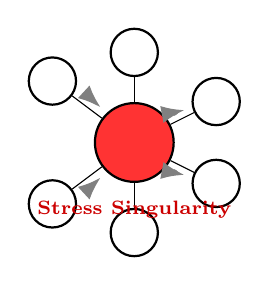
\begin{tikzpicture}[scale=0.52]
            \tikzstyle{node}=[circle, draw, thick, minimum size=6mm]
            \tikzstyle{hub}=[node, fill=red!80, minimum size=10mm]
            \tikzstyle{flow}=[-Latex, gray, thick, shorten <=1mm, shorten >=1mm]
            % Nodes
            \node[hub] (H) at (0,0) {};
            \node[node] (N1) at (2,1) {};
            \node[node] (N2) at (2,-1) {};
            \node[node] (N3) at (-2,1.5) {};
            \node[node] (N4) at (-2,-1.5) {};
            \node[node] (P1) at (0, 2.2) {};
            \node[node] (P2) at (0, -2.2) {};
            % Edges
            \draw (H) -- (N1); \draw (H) -- (N2);
            \draw (H) -- (N3); \draw (H) -- (N4);
            \draw (H) -- (P1); \draw (H) -- (P2);
            % Traffic Flows
            \draw[flow, line width=1.2pt] (N3) to [bend left=10] (H);
            \draw[flow, line width=1.2pt] (N4) to [bend right=10] (H);
            \draw[flow, line width=1.2pt] (H) to [bend left=10] (N1);
            \draw[flow, line width=1.2pt] (H) to [bend right=10] (N2);
            \node[below=0.1cm of H, text=red!80!black, font=\scriptsize\bfseries] {Stress Singularity};
        \end{tikzpicture}
    \end{minipage}
    }
    \hfill
    % ---- (b) After SRA ----
    \subfloat[SRA Control Paradigm: System Relaxation\label{fig:intro_after}]{%
    \begin{minipage}{0.46\columnwidth}
        \centering
        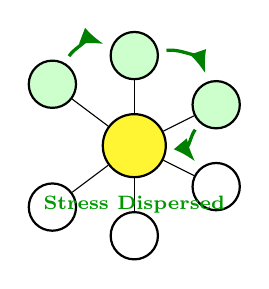
\begin{tikzpicture}[scale=0.52]
            \tikzstyle{node}=[circle, draw, thick, minimum size=6mm]
            \tikzstyle{hub}=[node, fill=yellow!80, minimum size=8mm]
            \tikzstyle{periph}=[node, fill=green!20]
            \tikzstyle{flow}=[-Latex, green!50!black, thick, shorten <=1mm, shorten >=1mm]
            % Nodes
            \node[hub] (H) at (0,0) {};
            \node[periph] (N1) at (2,1) {};
            \node[node] (N2) at (2,-1) {};
            \node[periph] (N3) at (-2,1.5) {};
            \node[node] (N4) at (-2,-1.5) {};
            \node[periph] (P1) at (0, 2.2) {};
            \node[node] (P2) at (0, -2.2) {};
            % Edges
            \draw (H) -- (N1); \draw (H) -- (N2);
            \draw (H) -- (N3); \draw (H) -- (N4);
            \draw (H) -- (P1); \draw (H) -- (P2);
            % Traffic Flows
            \draw[flow, line width=1.2pt] (N3) to [bend left=40] (P1);
            \draw[flow, line width=1.2pt] (P1) to [bend left=40] (N1);
            \draw[flow, line width=1.2pt] (N1) to [bend right=40] (N2);
            \node[below=0.1cm of H, text=green!60!black, font=\scriptsize\bfseries] {Stress Dispersed};
        \end{tikzpicture}
    \end{minipage}
    }
    
    \caption{Conceptual illustration of the core problem and the proposed SRA paradigm. SRA mitigates stress concentration by guiding the system toward a relaxed state of balanced load.}
    \label{fig:intro_scenario}
\end{figure}

The root of this fragility lies in a flawed focus on reactive symptoms rather than proactive structural governance. 
Prior work has largely attempted to patch this issue through \rev{three} dominant approaches, yet \rev{all} fall short of addressing the underlying cause:
\begin{itemize}
    \item \textbf{Reactive Load-Aware Routing (e.g., \cite{Macabale2020Cradle}):} These methods adjust paths based on transient metrics like queue length. They are essentially \textit{symptomatic treatments} that oscillate under high load due to delayed feedback loops.
    \item \rev{\textbf{Dynamic Link-Weight and Open-Loop Centrality Optimization (e.g., \cite{Fortz2000OSPF,Upadhyay2024OpticalBC}):} Classical IGP/OSPF weight tuning searches for link weights via combinatorial local search, while static centrality-based routing assigns one-shot penalties to high-betweenness nodes. When applied iteratively without state damping or temporal dwell regularization, instantaneous weight/centrality updates trigger severe route flapping across discontinuous shortest-path boundaries.}
    \item \textbf{Black-box AI Control (e.g., \cite{Wei2023GRLPS}):} While Deep Reinforcement Learning (DRL) agents can implicitly learn topology features, they function as uninterpretable ``black boxes,'' lacking the safety guarantees required for mission-critical infrastructure.
\end{itemize}

\rev{\textbf{Explicit Research Gap:} Despite extensive progress in traffic engineering, a critical theoretical and architectural gap remains: \textit{how to design a white-box, closed-loop supervisory control law that actively reshapes the routing cost landscape to disperse structural stress concentration, while mathematically guaranteeing global set attractivity, bounded tracking energy, and non-chattering practical stability across discontinuous shortest-path switching boundaries.} As summarized in Table~\ref{tab:related_work_comparison}, existing solutions fail to couple historical stress integration with temporal switching regularization.}

To bridge this gap, we propose a paradigm shift from reactive pathfinding to proactive \textit{stress governance}, inspired by the concept of ``relaxation'' in physical systems.
We introduce the System Relaxation Algorithm (SRA), a model-driven control system designed to disperse structural stress by dynamically reshaping the network's cost landscape.
Unlike black-box approaches, SRA operates as an interpretable, white-box dynamical system: it employs a ``leaky integrator'' mechanism \rev{coupled with a minimum dwell-time constraint} to accumulate historical stress into a controllable state variable, thereby guiding the network toward an emergent equilibrium of load balance (as conceptually illustrated in Fig.~\ref{fig:intro_scenario}).
Crucially, this control paradigm aligns perfectly with Software-Defined Networking (SDN) architectures, leveraging the controller's global view to calculate stress and its centralized authority to enforce the resulting cost policies \cite{hou2020reliable}.

\begin{table*}[t!]
\centering
\scriptsize\setlength{\tabcolsep}{4pt}\renewcommand{\arraystretch}{1.12}
\caption{\rev{Systematic Feature-by-Feature Comparison of Network Routing and Traffic Governance Paradigms}}
\label{tab:related_work_comparison}
\begin{tabularx}{\textwidth}{@{}l*{5}{>{\raggedright\arraybackslash}X}@{}}
\toprule
\textbf{Dimension} & \textbf{Reactive Queue-Aware \cite{Macabale2020Cradle,SM2025Novel}} & \textbf{Dynamic IGP Weight Tuning \cite{Fortz2000OSPF}} & \textbf{Static Centrality Optimization \cite{Upadhyay2024OpticalBC,DeMedeiros2017QuasiShortest}} & \textbf{AI / DRL-Based Routing \cite{Wei2023GRLPS,Feng2025MultiAgentGNN}} & \textbf{SRA (This Work)} \\
\midrule
\textbf{Sensing Signal} & Instantaneous local queue length / delay & Aggregate link utilization ratio & Static topological BC / degree & High-dimensional state embeddings & \rev{\textbf{Normalized topological or demand/capacity stress $\widetilde{\kappa}_i$}} \\
\textbf{Control Loop \& Memory} & Memoryless reactive feedback ($\alpha=1$) & Iterative combinatorial search & Open-loop one-shot static penalty & Black-box neural policy network & \rev{\textbf{Closed-loop leaky integrator ($\alpha \in (0,1)$)}} \\
\textbf{Anti-Chattering} & None (ping-pong oscillation) & Heuristic weight change limits & N/A (static weights) & Reward shaping only (no hard bound) & \rev{\textbf{Temporal dwell-time regularization ($T_d \ge 1$)}} \\
\textbf{Stability Proof} & None & None (NP-hard local search) & N/A & None (empirical convergence only) & \rev{\textbf{Krasovskii inclusion \& piecewise Lyapunov tube}} \\
\textbf{Hetero. Demand/Cap.} & Implicit via queue buildup & Supported via TM input & Neglected (topology-only) & Learned implicitly via training & \rev{\textbf{Explicitly supported via $\widetilde{\kappa}_i(S;W,\mu)$}} \\
\textbf{Per-Update Complexity} & $O(\text{deg}(i))$ local lookup & $O(I_{\text{search}}\cdot N(E+N\log N))$ & $O(N(E+N\log N))$ offline & $O(L_{\text{GNN}} E d^2)$ inference + training & \rev{\textbf{$O(N(E+N\log N))$ exact / $O(1)$ telemetry}} \\
\textbf{Interpretability} & High & Medium & High & Low (Black-box) & \textbf{High (White-box analytical law)} \\
\bottomrule
\end{tabularx}
\end{table*}

Our main contributions are summarized as follows:
\begin{enumerate}
    \item \textbf{A Unified Control-Theoretic Framework:} We formalize structural stress \rev{(both topological betweenness and demand/capacity-weighted load)} as a controllable state variable within a closed-loop dynamical system. \textbf{This framework explicitly decouples structural stress governance from low-level pathfinding}, treating conventional static routing \rev{($\alpha=0$) and memoryless reactive centrality routing ($\alpha=1$)} as degenerate boundary cases.
    
    \item \textbf{Rigorous Analysis of Discontinuous Dynamics:} We model discrete path switching in centrality-governed routing as a \textit{non-smooth dynamical system}. Using Krasovskii differential inclusions and piecewise Lyapunov functions, we provide formal proofs of \rev{global convergence to a compact invariant attracting set, bounded tracking energy under the Dissipation-Injection Law, and explicit peak-shaving capacity conditions}.
    
    \item \textbf{Topology-Dependent Intelligence \rev{and Comprehensive Validation}:} Through extensive simulations \rev{across BA, WS, ER, NSFNET, and GEANT topologies—including component ablations, stronger baselines, skewed/time-varying traffic, and sensing noise—}we demonstrate that SRA acts as a \textit{proactive performance optimizer} in heterogeneous networks and shifts to a \textit{resilience enhancement mechanism} in homogeneous networks.
\end{enumerate}

This work focuses on the algorithmic foundations and stability analysis of stress-aware network governance. 
While we discuss the alignment with SDN architectures, specific hardware implementations and south-bound protocol extensions are beyond the scope of this paper. The remainder of this paper is organized as follows: Section~\ref{sec:related_work} categorizes the existing literature and positions SRA within the routing landscape. 
Section~\ref{sec:model} establishes the unified theoretical framework, detailing the control-theoretic model, the rigorous stability analysis via non-smooth dynamics, and the formal bridge to capacity expansion. 
Section~\ref{sec:simulation} presents the empirical validation and analysis across the topological spectrum, and Section~\ref{sec:discussion_conclusion} concludes the paper.




\section{Related Work}
\label{sec:related_work}

The mitigation of structural stress remains a fundamental challenge at the intersection of network science and traffic engineering. While existing methodologies strive to balance traffic distribution, they vary significantly in their perception of network states and their subsequent control mechanisms. As synthesized in Table~\ref{tab:related_work_comparison}, there exists a discernible gap between traditional path-finding strategies and the active reshaping of a network's cost landscape. To situate the proposed System Relaxation Algorithm (SRA) within the broader research context, we categorize the existing literature into three distinct paradigms: reactive symptomatic management, static structural optimization, and black-box learning control.

\subsection{Reactive Control: Symptomatic Relief and Its Limitations}

The most pervasive paradigm in network control relies on \textit{reactive} feedback loops that adjust paths based on real-time performance metrics. These protocols typically monitor local queue lengths \cite{Macabale2020Cradle}, energy-aware load indicators \cite{SM2025Novel}, or composite link quality in highly dynamic satellite and vehicular environments \cite{Wang2025VANET, Fu2024SatelliteBC,wang2022cdmr}. For instance, the CRADLE protocol \cite{Macabale2020Cradle} leverages cross-layer cues to deflect traffic, while multi-criteria decision models \cite{Fouad2014MultiCriteria} and hierarchical cluster-based scaling \cite{Guizani2011Hierarchical} attempt to optimize routing decisions under fluctuating demands. Recent explorations in IoT and smart cities further extend this logic to position-based and occlusion-driven routing \cite{Darabkh2025SmartCity, Aditya2020ClosenessCluster}, addressing delays that often cascade across high-speed transport nodes \cite{Wu2024RailwayNode,ma2022traffic}.

While effective at mitigating immediate congestion, these methods essentially function as "symptom relievers" that address buffer overflows or link saturation rather than the underlying \textit{structural root causes}. By treating the network's cost landscape as an immutable constraint, reactive paradigms remain passive followers of instantaneous traffic noise. Consequently, they frequently suffer from the "ping-pong" effect—an instability where paths oscillate between overloaded and underloaded states due to delayed feedback. Lacking a long-term integration mechanism like SRA's leaky integrator, these approaches fail to distinguish between transient traffic spikes and endemic structural stress, and they lack the rigorous mathematical framework necessary to guarantee global stability under non-smooth traffic dynamics.

\subsection{Static Structural \rev{and IGP Weight} Optimization: The Open-Loop Governance Gap}

Recognizing the decisive role of network topology, a significant body of research leverages \rev{link-weight tuning \cite{Fortz2000OSPF} and} centrality metrics to guide routing and resource allocation. \rev{Classical IGP weight optimization \cite{Fortz2000OSPF} adjusts OSPF link weights using piecewise-linear convex congestion penalties via local search.} Betweenness Centrality (BC) \cite{Brandes2001Faster} and its sophisticated variants, such as link-variance optimization for optical networks \cite{Upadhyay2024OpticalBC} and weighted gravity models for multiplex systems \cite{Ni2023Gravity}, represent the established methodologies for identifying topological bottlenecks and influential nodes \cite{Basaras2019Influential, Wehmuth2021SpuriousPaths}. Theoretical advancements have further underscored that routing via quasi-shortest paths ($\rho$-geodesics) \cite{DeMedeiros2017QuasiShortest} or optimizing connectivity under probabilistic failures \cite{Cavallaro2022Connectivity} can significantly enhance network resilience. To circumvent the $O(N^3)$ computational complexity inherent in global centrality analysis, recent literature has proposed efficient approximation techniques, including hyperbolic space embeddings \cite{Stai2017Hyperbolic}, clustered parallelization \cite{Suppa2015FastBC}, and distributed estimation frameworks \cite{Maccari2020DistributedLoad, Maccari2018DistributedDV}. These structural insights have been applied across diverse domains, from optimizing SDN flow table storage \cite{Ma2019FlowTable} to enabling greedy forwarding in sparse networks \cite{Ahmed2025SparseNet} and energy-efficient path-finding in sensor networks \cite{Oliveira2010WSNcentrality}.

Despite their analytical depth, these structural optimization methods are fundamentally \textit{open-loop} and descriptive in nature. Even when accounting for temporal variations in centrality \cite{Ghanem2019DynamicCentrality}, the metrics are treated as passive observations rather than controllable state variables. \rev{When static centrality penalties or unregularized weight updates are applied repeatedly in closed loop, discrete shortest-path switching induces severe route oscillations.} Unlike SRA, these approaches lack a rigorous control-theoretic feedback law \rev{(combining leaky integration with dwell-time regularization)} to map structural observations into a provably stable cost landscape.

\subsection{AI-Driven and Self-Organizing Control: The Black-Box Dilemma}

The recent surge in machine learning has catalyzed the deployment of Deep Reinforcement Learning (DRL) and Graph Neural Networks (GNNs) for complex network management. State-of-the-art agents, such as GRL-PS \cite{Wei2023GRLPS} and multi-agent GNN frameworks \cite{Feng2025MultiAgentGNN}, attempt to implicitly capture topological features to navigate intricate congestion scenarios. To mitigate the computational overhead of global metrics, some approaches utilize node embeddings to approximate traditional centrality measures \cite{Mendonca2021ApproxCentrality}. Parallel to these learning-based methods, bio-inspired self-organizing models \cite{Cheng2010SelfOrganizingModel, Guo2010HybridSelfOrg, Li2014PhysarumMulticast} and heuristic search strategies—including discrete particle swarm optimization \cite{Wang2019DPSO} and genetic algorithms \cite{Mu2024CarrierSelfOrg}—have been applied to dynamic cluster-based routing. These autonomous path-finding capabilities are particularly explored in mission-critical environments such as missile swarm networks \cite{Lu2022MissileSwarm,ma2021credibility}, where nodes must adapt to rapid topology changes.

Despite their empirical performance, these approaches frequently operate as \textit{black boxes} with opaque decision logic. They generally lack formal safety verification or rigorous Lyapunov stability guarantees, posing systemic risks to critical infrastructure where the unpredictable convergence of DRL agents remains a significant concern. Furthermore, heuristic and self-organizing models often overlook the non-smooth discontinuities inherent in discrete path-switching actions. This theoretical void is bridged by SRA, which provides a "white-box" alternative through the rigorous application of non-smooth dynamical systems theory \cite{Aubin1984Differential}, ensuring both mathematical explainability and guaranteed global convergence.

In summary, while the aforementioned paradigms have significantly advanced network engineering, a fundamental gap persists between topological awareness and active governance. Reactive methods prioritize speed over stability, static structural optimizations offer diagnostic depth but lack execution mechanisms, and learning-based controls trade mathematical explainability for empirical performance. Specifically, the networking community still lacks a unified framework that can bridge the "governance gap" between high-level structural observations (centrality) and low-level traffic control laws with guaranteed global stability. This paper addresses these limitations by introducing the System Relaxation Algorithm (SRA). By grounding the control logic in non-smooth dynamical systems theory and the "Cost Law" mechanism, SRA transitions the network management philosophy from passive path-finding to the active, stable, and explainable reshaping of the network's cost landscape.

\section{Theoretical Model and Methods}
\label{sec:model}

We formulate the problem of stress-aware network governance not as a sequence of heuristic routing updates, but as a \textbf{discrete-time, non-smooth dynamical system}. 
This control-theoretic perspective is decisive: it allows us to transcend the stability pitfalls of naive reactive protocols, which often collapse into destructive oscillations due to their lack of system memory.
In our framework, the network's cost landscape is no longer a static input, but a dynamic state variable governed by a physics-inspired ``leaky integrator.''
This section provides a systematic construction of this system. 
We first define the network model and formalize structural stress as a controllable state. 
We then detail the core state evolution law that couples continuous stress accumulation with discrete path switching. 
The culmination is a rigorous analysis using piecewise Lyapunov functions and discrete-time inclusion theory, proving that SRA guarantees global convergence to a \rev{compact invariant attracting set}---a theoretical guarantee that heuristic methods fundamentally lack.

\subsection{Network Model, \rev{Generalized Stress Metric, and Problem Formulation}}

We model the underlying network topology as a connected undirected graph $G=(V,E)$ with $N=|V| \ge 3$ nodes. 
From a control perspective, the network's ``plant'' is governed by a dynamically evolving node cost vector $C \in \mathbb{R}^N_+$. 
This vector defines the instantaneous \textit{cost landscape}, where the cost of any path $P$ is the sum of the transit costs of its constituent nodes, i.e., $d(P) = \sum_{v \in P} C_v$. 
Traffic flows are assumed to follow lowest-cost paths within this landscape.

\rev{To ensure mathematical transparency, our control model operates under four explicit structural and operational assumptions:
\begin{itemize}
    \item \textbf{Assumption 1 (2-Vertex-Connected Core / Alternative Paths):} For bottleneck nodes of interest, the graph $G$ contains at least two vertex-disjoint simple paths between major source-destination pairs (for true cut-vertices or bridges, structural stress is physically irreducible; see Section~\ref{subsec:limitations}).
    \item \textbf{Assumption 2 (Time-Scale Separation):} Control-plane cost updates occur at discrete epochs $k \in \mathbb{N}$ on a slower time scale than data-plane packet forwarding, allowing path-level flow rates to reach quasi-stationary equilibrium within each control epoch.
    \item \textbf{Assumption 3 (Equal-Cost Shortest-Path Splitting / Finite Configurations):} Equal-cost shortest paths between any origin-destination pair $(s,t)$ split flow equally across the active shortest-path set (or follow a fixed tie-breaking rule on an arbitrarily small tie perturbation), guaranteeing that the family of realizable shortest-path configurations $\mathcal{P}$ on any finite graph $G$ is finite ($|\mathcal{P}| = M < \infty$).
    \item \textbf{Assumption 4 (Quasi-Stationary Demand and Service Capacity):} Over a relaxation horizon, each origin-destination (OD) pair $(s,t)$ has a non-negative relative traffic weight $W_{st} \ge 0$, and each node $i \in V$ has an effective transit service capacity $\mu_i > 0$.
\end{itemize}}

To quantify the structural stress induced by a specific cost distribution, we employ \textbf{Betweenness Centrality (BC)} \cite{Brandes2001Faster} as the baseline topological feedback signal. 
The unnormalized topological stress on node $i$, denoted $\kappa_i(S)$, represents its absolute path load under uniform unit demand ($W_{st} \equiv 1$):
\begin{equation}
    \label{eq:bc_definition}
    \kappa_i(S) = \sum_{s\neq i\neq t\in V} \frac{\sigma^{\,C(S)}_{st}(i)}{\sigma^{\,C(S)}_{st}}
\end{equation}
where $\sigma^{\,C(S)}_{st}$ is the total number of shortest paths between $s$ and $t$ under the cost configuration $C(S)$, and $\sigma^{\,C(S)}_{st}(i)$ is the subset passing through $i$.

\rev{Furthermore, to address non-uniform traffic matrices $W = [W_{st}]$ and heterogeneous node service capacities $\mu = (\mu_i)_{i \in V}$, we generalize Eq.~\eqref{eq:bc_definition} to the \textbf{Demand- and Capacity-Weighted Structural Stress}:
\begin{equation}
    \label{eq:generalized_stress}
    \widetilde{\kappa}_i(S; W, \mu) := \frac{1}{\mu_i} \sum_{s\neq i\neq t\in V} W_{st}\,\frac{\sigma^{\,C(S)}_{st}(i)}{\sigma^{\,C(S)}_{st}}.
\end{equation}
When demands are uniform ($W_{st}\equiv 1$) and node capacities are homogeneous ($\mu_i \equiv \mu$), $\widetilde{\kappa}_i(S; W, \mu)$ reduces to $\kappa_i(S)/\mu$, whose max-normalization is identical to that of topological BC in Eq.~\eqref{eq:bc_definition}. Crucially, because $W_{st}$ and $\mu_i$ are constants within a control horizon, $\widetilde{\kappa}(S; W, \mu)$ remains piecewise constant over the same finite partition of the state space $X=[0,1]^N$, so all subsequent stability proofs hold identically for both $\kappa(S)$ and $\widetilde{\kappa}(S; W, \mu)$.}

Since $\kappa_i(S)$ is unbounded with network size, we project this feedback signal into a compact state space to ensure system stability. 
We define the max-normalized stress vector as:
\begin{equation}
    \label{eq:bc_normalization}
    \kappa_{\max}(S):=\max_j\kappa_j(S).
\end{equation}
\begin{equation}
    \mathrm{norm}(\kappa(S)) =
    \begin{cases}
    \displaystyle \frac{\kappa(S)}{\kappa_{\max}(S)}, & \text{if } \kappa_{\max}(S) > 0,\\[6pt]
    \mathbf{0}, & \text{otherwise.}
    \end{cases}
\end{equation}
This normalization confines the feedback signal strictly within the unit hypercube $[0,1]^N$. 
\textbf{Key Geometric Property:} Crucially, for any finite graph, the set of all possible shortest-path configurations (including boundary tie subsets) is finite. 
This implies that $\mathrm{norm}(\kappa(S))$ does not vary continuously but jumps between a \textbf{finite set of constant vectors} \rev{$\{v_1, \dots, v_M\} \subset [0,1]^N$}. 
This quantization is non-trivial; it renders the system dynamics \textit{piecewise constant}, forming the topological foundation for our non-smooth convergence analysis in Section~\ref{sec:convergence_analysis}.

\rev{\textbf{Formal Problem Formulation:} Formally, given $(G, W, \mu)$, we seek a closed-loop state feedback policy mapping historical stress observations $\{\kappa^{(0)}, \dots, \kappa^{(k)}\}$ to node transit costs $C^{(k+1)} \in [1, 1+\beta_I]^N$ so as to solve the bi-criteria resilient governance problem (with switching-cost weight $\eta_{\text{sw}} \ge 0$):
\begin{equation}
    \label{eq:problem_formulation}
    \begin{aligned}
    \min_{\{S^{(k)}, C^{(k)}\}} \quad & \limsup_{k \to \infty} \max_{i \in V} \widetilde{\kappa}_i(S^{(k)}; W, \mu) + \eta_{\text{sw}}\,\bar{f}_{\text{sw}} \\
    \text{s.t.} \quad & S^{(k+1)} = (1-\alpha)S^{(k)} + \alpha\,q^{(k)},\quad S^{(0)} \in [0,1]^N, \\
    & C^{(k)} = \mathbf{1} + \beta_I S^{(k)}, \quad \tau_{m+1} - \tau_m \ge T_d, \\
    & \bar{f}_{\text{sw}} \le 1/T_d,
    \end{aligned}
\end{equation}
where $\bar{f}_{\text{sw}} := \limsup_{K\to\infty}\frac{1}{K}\sum_{k=0}^{K-1}\mathbb{I}(\mathcal{P}^{(k+1)}\neq\mathcal{P}^{(k)})$ is the asymptotic switching frequency, $\mathcal{P}^{(k)}$ denotes the active shortest-path configuration at step $k$, $\{\tau_m\}$ are the route-switching epochs separated by at least the minimum dwell time $T_d \ge 1$.}

% --- 这是 Fig. 2 的完整代码 ---
\begin{figure*}[!t]
    \centering
    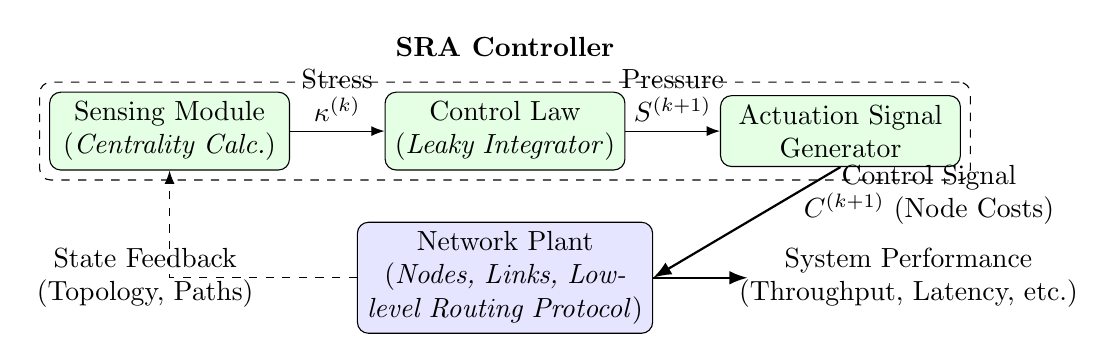
\begin{tikzpicture}[
        auto,
        node distance=0.65cm and 1.2cm,
        plant/.style={rectangle, draw, fill=blue!10, text width=10em, text centered, rounded corners, minimum height=2.4em},
        module/.style={rectangle, draw, fill=green!10, rounded corners, text width=8em, text centered, minimum height=2.4em},
        line/.style={draw, -{Latex}},
        signal/.style={draw, -{Latex}, thick},
        feedback/.style={draw, -{Latex}, dashed}
    ]
    % SRA Controller's Internal Modules
    \node [module] (sensing) {Sensing Module \\ (\textit{Centrality Calc.})};
    \node [module, right=of sensing] (law) {Control Law \\ (\textit{Leaky Integrator})};
    \node [module, right=of law] (actuation) {Actuation Signal Generator};
    % Network Plant
    \node [plant, below=of law] (plant) {Network Plant \\ (\textit{Nodes, Links, Low-level Routing Protocol})};
    % Dashed container for the SRA controller
    \node [draw, rounded corners, fit=(sensing) (law) (actuation), label={[yshift=0.2cm]above:\textbf{SRA Controller}}, inner sep=0.12cm, dashed] (controller_box) {};
    % Connections
    \path [signal] (actuation.south) -- node [right, pos=0.25, align=center] {Control Signal \\ $C^{(k+1)}$ (Node Costs)} (plant.east);
    \path [feedback] (plant.west) -| node [left, pos=0.25, align=center] {State Feedback \\ (Topology, Paths)} (sensing.south);
    % Internal Controller Connections
    \path [line] (sensing.east) -- node [above, align=center] {Stress \\ $\kappa^{(k)}$} (law.west);
    \path [line] (law.east) -- node [above, align=center] {Pressure \\ $S^{(k+1)}$} (actuation.west);
    % System Performance Output
    \coordinate[right=of plant] (output_coord);
    \path [signal] (plant.east) -- node [right, pos=0.8, align=center] {System Performance \\ (Throughput, Latency, etc.)} (output_coord);
    \end{tikzpicture}
    \caption{The architecture of the SRA as a closed-loop control system. The SRA controller acts as a supervisory layer that governs the underlying network plant by dynamically adjusting the cost landscape.}
    \label{fig:sra_architecture}
\end{figure*}

\subsection{SRA: Core Mechanism and Algorithm Implementation}
\label{subsec:sra_mechanism}

\textit{Supervisory Closed-Loop Architecture.} 
SRA operates as a supervisory governance layer (Fig.~\ref{fig:sra_architecture}) that reshapes the node cost landscape upon which standard routing protocols (e.g., OSPF, IS-IS, or Dijkstra) execute. Setting node costs directly proportional to instantaneous centrality creates an unstable ``bang-bang'' feedback loop. To dampen high-frequency fluctuations, SRA introduces a \textbf{leaky integrator} state vector---the accumulated pressure $S \in \mathbb{R}^N_+$---which evolves as:
\begin{equation}
    \label{eq:pressure_update}
    S_i^{(k+1)} = (1 - \alpha) S_i^{(k)} + \alpha \cdot \mathrm{norm}(\kappa_i^{(k)})
\end{equation}
where $k$ is the iteration step and $\alpha \in (0,1)$ governs memory persistence. Physically, Eq.~\eqref{eq:pressure_update} acts as a digital low-pass filter with damping factor $(1-\alpha)$.

\begin{remark}[Relationship to Reactive Routing]
\label{rem:reactive_routing}
Standard memoryless reactive routing corresponds to the degenerate boundary case $\alpha=1$ in Eq.~\eqref{eq:pressure_update}, where the damping term $(1-\alpha)$ vanishes.
\end{remark}

The node transit cost $C$ is then defined via an affine control law:
\begin{equation}
    \label{eq:cost_update}
    C_i^{(k+1)} = 1 + \beta_I \cdot S_i^{(k+1)}
\end{equation}
where $1$ is the base physical cost and $\beta_I > 0$ is the pressure-to-cost gain factor.

% --- Fig. 3 Code Remains Unchanged ---
\begin{figure}[!t]
    \centering
    \includegraphics[width=0.68\columnwidth]{fig3xunhuan.eps}
    \caption{The iterative workflow of the SRA control loop, illustrating the four key phases of sensing, decision-making, actuation, and system influence that drive the network toward a state of dispersed structural stress.}
    \label{fig:sra_workflow}
\end{figure}

The complete procedure is formalized in Algorithm~\ref{alg:sra} (Fig.~\ref{fig:sra_workflow}), which incorporates a minimum dwell time $T_d \ge 1$ to prevent immediate self-perturbation and diverts flows from congested hubs to peripheral detours (Fig.~\ref{fig:sra_mechanism_visualization}).

% --- 这是 Algorithm 1 的完整代码 ---
\begin{breakablealgorithm}
\caption{System Relaxation Algorithm (SRA)}
\label{alg:sra}
{\footnotesize
\begin{algorithmic}[1]
\REQUIRE Graph $G=(V,E)$; \rev{optional demand weights $W=[W_{st}]$ and node service rates $\mu=(\mu_i)$}; learning rate $\alpha \in (0,1)$; pressure-cost factor $\beta_I > 0$; stopping threshold $\varepsilon > 0$; max iterations $K_{\max}$; minimum dwell time $T_d \ge 1$.
\ENSURE \rev{Final node cost vector $C^{(k)}$ and active routing policy $\mathcal{P}^{(k)}$.}
\STATE Initialize $S^{(0)} \leftarrow \mathbf{0}$, $C^{(0)} \leftarrow \mathbf{1}$, \rev{and dwell counter $\tau_{\text{dwell}} \leftarrow 0$}.
\FOR{$k=0,1,2,\ldots,K_{\max}-1$}
\STATE \rev{\textbf{if} $\tau_{\text{dwell}} == 0$ \textbf{then}}
\STATE \quad \rev{Compute all-pairs shortest-path DAGs $\mathcal{P}^{(k)}$ and stress $\kappa^{(k)}$ (Eq.~\eqref{eq:bc_definition} or $\widetilde{\kappa}^{(k)}$ in Eq.~\eqref{eq:generalized_stress}) via Brandes' algorithm under $C^{(k)}$; set $q^{(k)} \leftarrow \mathrm{norm}(\kappa^{(k)})$ and $\tau_{\text{dwell}} \leftarrow T_d - 1$ ($\triangleright\; O(N(E+N\log N))$).}
\STATE \rev{\textbf{else}}
\STATE \quad \rev{Hold active routing policy and stress target: $\mathcal{P}^{(k)} \leftarrow \mathcal{P}^{(k-1)}$, $q^{(k)} \leftarrow q^{(k-1)}$, and $\tau_{\text{dwell}} \leftarrow \tau_{\text{dwell}} - 1$ ($\triangleright\; O(N)$).}
\STATE \rev{\textbf{end if}}
\STATE Update pressure: $S^{(k+1)} \leftarrow (1-\alpha)S^{(k)}+\alpha\,q^{(k)}$ \rev{($\triangleright\; O(N)$)}.
\STATE Update cost: $C^{(k+1)} \leftarrow \mathbf{1}+\beta_I\,S^{(k+1)}$ \rev{($\triangleright\; O(N)$)}.
\IF{\rev{$k > 0$ and $\|S^{(k+1)}-S^{(k)}\|_\infty \le \varepsilon$ and $\mathcal{P}^{(k)} == \mathcal{P}^{(k-1)}$}}
\STATE \textbf{break}
\ENDIF
\ENDFOR
\RETURN \rev{$C^{(k)}, \mathcal{P}^{(k)}$}
\end{algorithmic}
}
\end{breakablealgorithm}

% --- 这是 Fig. 4 (原文fig 7) 的代码 ---
\begin{figure}[!t]
    \centering
    \includegraphics[width=0.68\columnwidth]{figure_7_microscopic_path_change.eps}
    \caption{A conceptual visualization of SRA's path reshaping mechanism. The algorithm diverts traffic from the efficient but congested 2-hop path (red dashed) through the central hub to a longer but more stable 4-hop peripheral path (green solid).}
    \label{fig:sra_mechanism_visualization}
\end{figure}

\subsection*{Complexity and Scalability Analysis}

A full centrality evaluation in SRA uses Brandes' algorithm \cite{Brandes2001Faster}, requiring $O(N(E + N \log N))$ time and $O(N + E)$ working memory per source traversal \rev{(plus $O(N^2)$ routing-table storage). When dwell-time gating $T_d > 1$ is active, Brandes' recomputation executes only at block boundaries $\tau_m = m T_d$, while the $T_d - 1$ intra-block cooling steps reuse $q^{(\tau_m)}$ in $O(N)$ time, yielding an amortized complexity of $O(N(E + N \log N)/T_d + N)$ per epoch ($31.17$~ms per evaluation at $N=100$ and $850.99$~ms at $N=500$; see Section~\ref{subsec:scalability_eval}).} For hyper-scale deployments, nodes can approximate local stress in $O(1)$ per-packet time by counting transiting flows weighted by $1/\mu_i$ \cite{Maccari2020DistributedLoad} via OSPF-TE or SDN In-band Network Telemetry (INT).

\subsection{Global Attractiveness and Existence Guarantee for Convergence}
\label{sec:convergence_analysis}
\label{subsec:attractivity}

Because shortest-path routing switches discontinuously across polyhedral boundaries, we analyze the hybrid dynamics using discrete-time differential inclusions \cite{Aubin1984Differential}. Under $T_d=1$ (or at block boundaries $\tau_m = m T_d$ with effective step size $\alpha_{T_d} = 1 - (1-\alpha)^{T_d} \in (0,1)$), the state evolution on $X = [0,1]^N$ is governed by the set-valued map:
\begin{equation}\label{eq:inclusion_map}
S^{(k+1)} \in F(S^{(k)}) := (1-\alpha)S^{(k)}+\alpha\,\mathcal{N}(S^{(k)})
\end{equation}
where $\mathcal{N}(S) := \bigcap_{\delta > 0} \overline{\mathrm{co}}\big(\mathrm{norm}(\kappa(B_\delta(S)))\big)$ is the \textbf{Krasovskii regularization} of the discontinuous mapping $\mathrm{norm}(\kappa(\cdot))$. 
Geometrically, this operation takes the closed convex hull of all limit points in a vanishing neighborhood of $S$, effectively ``filling in the gaps'' caused by discrete routing decisions (including multi-path tie boundaries). 
This yields a mathematically well-behaved map, allowing us to derive the following foundational properties.

\begin{lemma}[Global Confinement and Safety]
\label{lemma:invariance}
Let the state space be the unit hypercube $X=[0,1]^N$. 
The discrete-time inclusion for SRA, given by $S^{(k+1)}\in F(S^{(k)})$, is strictly confined within $X$. 
Formally, $X$ is a \textbf{compact, positively invariant set} ($F(X) \subset X$) and is \rev{exponentially attracting for any out-of-bounds perturbation $S^{(0)} \in [-1/\beta_I + \epsilon, \infty)^N$}.
\textit{Physical Interpretation:} This lemma guarantees that the structural stress never diverges to infinity; the system possesses an intrinsic ``safety boundary'' dictated by the normalization mechanism.
\end{lemma}
\begin{proof}[Proof Sketch]
The proof demonstrates that if a state $S^{(k)}$ resides within the hypercube $X$, its successor $S^{(k+1)}$---being a convex combination of elements in $X$---must inherently remain within $X$. Moreover, for any perturbed initialization $S^{(0)} \notin X$, the $\ell_\infty$ distance to $X$ contracts geometrically by $(1-\alpha)$ at every step. \textit{The complete step-by-step formal proof is provided in Supplementary Material Section S-A.}
\end{proof}

With safety guaranteed, we verify the topological regularity of the control map.

\begin{proposition}[Topological Regularity]
\label{prop:usc}
The set-valued map $F(\cdot)$ defined in \eqref{eq:inclusion_map} is \textbf{Upper Semi-Continuous (USC)} with \textbf{non-empty, compact, and convex} values.
\end{proposition}
\begin{proof}[Proof Sketch]
The proof exploits the piecewise constant structure of $\mathcal{N}(S)$, which stems from the finite nature of the network's path configurations (Assumption 3). This structure ensures that the graph of the map is closed, a sufficient condition for the USC property in compact spaces. \textit{The complete step-by-step formal proof is provided in Supplementary Material Section S-B.}
\end{proof}

Combining the global confinement (Lemma~\ref{lemma:invariance}) with topological regularity (Proposition~\ref{prop:usc}), we establish the system's ultimate destiny.

\begin{theorem}[\rev{Global Convergence to a Compact Invariant Attracting Set}]
\label{thm:attractor}
For the discrete-time inclusion \eqref{eq:inclusion_map}, the nested intersection
\begin{equation}\label{eq:omega_nested_def}
\rev{\Omega := \bigcap_{n=0}^{\infty} F^n(X) \subset X:=[0,1]^N}
\end{equation}
is a \textbf{non-empty, compact, and positively invariant global attracting set} ($F(\Omega)=\Omega$), such that for any initial configuration $S^{(0)}\in X$:
\begin{equation}\label{eq:attractor_convergence}
\mathrm{dist}\big(S^{(k)},\Omega\big)\ \to\ 0\qquad (k\to\infty).
\end{equation}
\end{theorem}
\begin{proof}[Proof Sketch]
Because $X$ is compact and positively invariant ($F(X) \subset X$) and $F$ is USC with compact values (Proposition~\ref{prop:usc}), the forward images $K_n := F^n(X)$ form a nested sequence of non-empty compact subsets $K_{n+1} \subset K_n$. By Cantor's intersection theorem, $\Omega = \bigcap_{n\ge 0} K_n$ is non-empty, compact, and invariant, and attracts all trajectories initialized in $X$. \textit{The complete step-by-step formal proof is provided in Supplementary Material Section S-C.}
\end{proof}

\rev{\begin{remark}[Attraction to a Limit Set vs. Unique Point Equilibrium]
\label{rem:attractor_vs_unique}
We emphasize that Theorem~\ref{thm:attractor} guarantees global convergence to a \textit{compact invariant set} $\Omega$ rather than a single static fixed point $S^\star$. In non-smooth routing systems where shortest-path trees switch discontinuously across polyhedral partition boundaries, a unique static fixed point does not generally exist unless a single routing configuration is self-consistent in the interior of its partition cell (Corollary~\ref{cor:local_convergence}). Otherwise, trajectories are attracted to bounded invariant orbits (such as multi-path switching cycles) within $\Omega$, whose tracking-energy radius is explicitly bounded by the Dissipation-Injection Law (Theorem~\ref{thm:drop_jump}) and contracted by the minimum dwell time $T_d$ (Theorem~\ref{thm:epsilon_tube}).
\end{remark}}

\subsection{Energy Dissipation and Bounded Oscillation Analysis}
\label{subsec:lyapunov}

While the existence of a global attracting set $\Omega$ guarantees safety, it does not quantitatively bound the amplitude of steady-state oscillations across switching boundaries. 
To rigorously characterize the system's steady-state dynamics, we introduce a specialized analytical tool from non-smooth mechanics: the \textbf{piecewise Lyapunov tracking function}.
\rev{At any iteration $k$, let $q^{(k)} := \mathrm{norm}(\kappa^{(k)}) \in [0,1]^N$ denote the active normalized stress vector driving the state update $S^{(k+1)} = (1-\alpha)S^{(k)} + \alpha q^{(k)}$ in Algorithm~\ref{alg:sra}. We define the instantaneous tracking energy $E_k$ and the set-distance function $V(S)$ as:
\begin{equation}\label{eq:lyapunov_def}
E_k := \|S^{(k)} - q^{(k)}\|_2^2, \qquad V(S) := \min_{c\in\mathcal N(S)}\|S-c\|_2^2.
\end{equation}
Whenever $q^{(k)} \in \mathcal{N}(S^{(k)})$ (which holds at every step when $T_d=1$ and at every block-onset recomputation step $k=\tau_m$ when $T_d > 1$), we have $V(S^{(k)}) \le E_k$, with exact equality $V(S^{(k)}) = E_k$ in the interior of each routing partition where $\mathcal{N}(S^{(k)}) = \{q^{(k)}\}$.}
Let $\bar{\Delta} := \max_{\ell, m} \|v_\ell - v_m\|_2$ denote the maximum Euclidean diameter of the finite set of normalized centrality vectors $\{v_1, \dots, v_M\}$, representing the worst-case topological shock. 
The following theorem reveals the fundamental \textit{thermodynamics} of the SRA control loop.

\begin{theorem}[The Dissipation-Injection Law]
\label{thm:drop_jump}
\rev{For any iteration $k$ of the SRA dynamics $S^{(k+1)} = (1-\alpha)S^{(k)} + \alpha q^{(k)}$ with active target $q^{(k)} \in \{v_1, \dots, v_M\}$, the tracking energy $E_k = \|S^{(k)} - q^{(k)}\|_2^2$ satisfies the exact one-step dissipation-injection inequality:
\begin{equation}\label{eq:drop_jump_one_step}
\begin{aligned}
E_{k+1} &\le (1-\alpha)\,E_k + \frac{1}{\alpha}\,\|q^{(k)} - q^{(k+1)}\|_2^2 \\
&\le \underbrace{(1-\alpha)\,E_k}_{\text{Dissipation (Drop)}}\ +\ \underbrace{\dfrac{1}{\alpha}\,\bar\Delta^{2}}_{\text{Injection (Jump)}}.
\end{aligned}
\end{equation}
In particular, whenever the active path set does not change between steps $k$ and $k+1$ ($q^{(k+1)} = q^{(k)}$), the injection term vanishes identically and $E_{k+1} = (1-\alpha)^2 E_k \le (1-\alpha) E_k$. Consequently, $E_k$ (and $V(S^{(k)}) \le E_k$ at all recomputation epochs) is ultimately bounded, satisfying:}
\begin{equation}\label{eq:limsup_boundedness}
\rev{\limsup_{k\to\infty} E_k\ \le\ \frac{\bar\Delta^{2}}{\alpha^2}.}
\end{equation}
\end{theorem}
\begin{proof}[Proof Sketch]
Using the exact identity $S^{(k+1)} - q^{(k+1)} = (1-\alpha)(S^{(k)} - q^{(k)}) + (q^{(k)} - q^{(k+1)})$ and applying the Weighted Young's Inequality with weight $\lambda = \alpha/(1-\alpha)$, we decouple the one-step evolution into a contractive dissipation term $(1-\alpha)E_k$ and a switching disturbance term $\frac{1}{\alpha}\|q^{(k)} - q^{(k+1)}\|_2^2 \le \frac{1}{\alpha}\bar{\Delta}^2$. \textit{The complete step-by-step formal proof is provided in Supplementary Material Section S-D.}
\end{proof}

This theorem provides a profound physical insight: the stability of SRA is governed by two competing forces. 
The \textbf{Dissipation Term} (Drop) represents the damping effect of the leaky integrator, continuously draining energy from the system with a contraction factor of $(1-\alpha)$. 
The \textbf{Injection Term} (Jump) represents the energy injected by discrete topological switching. 
Stability is achieved because the injection is bounded by $\bar{\Delta}^2$, ensuring the system settles into a low-energy orbit rather than diverging.

To further validate the choice of the leaky integrator, we consider the local regime where the topology stabilizes.

\begin{corollary}[Ideal Linear Convergence]
\label{cor:local_convergence}
In the local regime where the shortest-path set remains constant ($q^{(k)} \equiv c$), the injection term vanishes. The update rule simplifies to a linear contraction map:
\begin{equation}\label{eq:linear_update}
S^{(k+1)}=(1-\alpha)S^{(k)}+\alpha c,
\end{equation}
which converges exponentially to the unique fixed point $S^\star=c$ at a rate of $(1-\alpha)$.
\end{corollary}
\begin{proof}[Proof Sketch]
The proof follows directly from the Banach Fixed-Point Theorem. By subtracting the fixed point from the update rule, we derive the linear error dynamics $\|S^{(k+1)}-S^\star\|_2 = (1-\alpha)\|S^{(k)}-S^\star\|_2$, confirming exponential decay. \textit{The complete step-by-step formal proof is provided in Supplementary Material Section S-E.}
\end{proof}

\subsection{Convergence Rate and Practical Stability via Temporal Regularization}
\label{subsec:practical_stability_rate}

The ``Dissipation-Injection'' law (Theorem~\ref{thm:drop_jump}) guarantees that the system energy is ultimately bounded. 
However, to bridge the gap between mathematical boundedness and engineering utility, two critical questions remain: \textit{At what rate} does the system relax to this bounded orbit, and how can we systematically suppress high-frequency \textit{route chattering}?
We address these by introducing a \textbf{minimum dwell time, $T_d$}, as a rigorous \textbf{temporal regularization} for the hybrid dynamics.
By decomposing the system's evolution into distinct ``dwell blocks'' of length $T_d$ in Algorithm~\ref{alg:sra}, we derive explicit convergence rates and a tunable stability guarantee.

We define the $m$-th dwell block as the interval $[\tau_m, \tau_{m+1}-1]$, where $\tau_m = m T_d$ and $\tau_{m+1} = \tau_m + T_d$. 
\rev{Let $S_m := S^{(\tau_m)}$ and $V_m := E_{\tau_m} = \|S^{(\tau_m)} - q^{(\tau_m)}\|_2^2$ denote the state and tracking energy at the onset of block $m$ (where $q^{(\tau_m)} \in \mathcal{N}(S^{(\tau_m)})$, so $V(S_m) \le V_m$).}

\begin{proposition}[Block-wise Dissipation Dynamics]
\label{prop:block_dynamics}
Under the temporal regularization $T_d$ in Algorithm~\ref{alg:sra}, the active routing topology and target vector $q^{(\tau_m+t)} \equiv q^{(\tau_m)}$ remain invariant within each block $t \in \{0, \dots, T_d-1\}$. 
Letting $\gamma:=1-\alpha$ be the damping factor and $\tilde C:=\bar\Delta^2/\alpha$ be the injection bound, the system exhibits a \textbf{contract-then-jump} behavior:
\begin{itemize}
    \item[\textit{(i)}] \textbf{Intra-block Cooling:} Within a block, the injection term vanishes ($q^{(\tau_m+t)} = q^{(\tau_m)}$), and tracking energy decays exponentially for $t \in \{0, \dots, T_d-1\}$:
    \begin{equation}\label{eq:intra_block}
    \rev{E_{\tau_m+t} = \gamma^{\,2t}V_m \le \gamma^{\,t}V_m.}
    \end{equation}
    \item[\textit{(ii)}] \textbf{Inter-block Recurrence:} The energy state across adjacent blocks satisfies the linear recurrence:
    \begin{equation}\label{eq:inter_block}
    V_{m+1}\ \le\ \gamma^{T_d}\,V_m\ +\ \tilde C.
    \end{equation}
\end{itemize}
\end{proposition}
\begin{proof}[Proof Sketch]
(i) During the dwell period, the path set is held fixed ($q^{(\tau_m+t)} \equiv q^{(\tau_m)}$), so the system operates as a pure leaky integrator (Corollary~\ref{cor:local_convergence}), resulting in strictly exponential decay. (ii) The recurrence combines $T_d-1$ steps of intra-block cooling with a single worst-case switching injection event at the block boundary $\tau_{m+1}$. \textit{The complete step-by-step formal proof is provided in Supplementary Material Section S-F.}
\end{proof}

This recurrence relation allows us to calculate the precise geometry of the system's final resting state.

\begin{theorem}[Tunable Convergence to an $\varepsilon$-Attractor]
\label{thm:epsilon_tube}
Let $\gamma \in (0,1)$ and $\tilde C > 0$. The system trajectories are strictly confined as follows:
\begin{itemize}
    \item[\textit{(a)}] \textbf{Steady-State Radius:} The block-onset energy ultimately converges into a bounded tube of radius:
    \begin{equation}\label{eq:limsup_radius}
    \limsup_{m\to\infty}V_m\ \le\ \frac{\tilde C}{1-\gamma^{T_d}}.
    \end{equation}
    \item[\textit{(b)}] \textbf{Finite-Time Entry:} For any target radius $\varepsilon^2 > \frac{\tilde C}{1-\gamma^{T_d}}$, the system enters the $\varepsilon$-tube ($V_m \le \varepsilon^2$) in a finite number of blocks $m \ge M(\varepsilon)$, explicitly bounded by $M(\varepsilon)=0$ when $V_0 \le \varepsilon^2 - \frac{\tilde C}{1-\gamma^{T_d}}$ and otherwise by:
    \begin{equation}\label{eq:finite_time_blocks}
    \rev{M(\varepsilon) := \left\lceil \frac{\ln\!\big((\varepsilon^2 - \frac{\tilde C}{1-\gamma^{T_d}})/V_0\big)}{T_d \ln \gamma} \right\rceil.}
    \end{equation}
\end{itemize}
\end{theorem}
\begin{proof}[Proof Sketch]
We iteratively expand the recurrence from Proposition~\ref{prop:block_dynamics}. The energy $V_m$ is upper-bounded by a geometric series which converges to the stated limit. \textit{The complete step-by-step formal proof is provided in Supplementary Material Section S-G.}
\end{proof}

Finally, we consolidate these findings into a definitive stability guarantee.

\begin{theorem}[The Practical Stability Guarantee]
\label{thm:practical_stability}
With a minimum dwell time $T_d \ge 1$, the SRA framework guarantees:
\begin{itemize}
    \item[\textit{(a)}] \textbf{Suppression of High-Frequency Chattering:} \rev{The number of route switches over any $T$-step horizon satisfies $N_{\text{sw}}(T) \le \lceil T/T_d \rceil$, so the asymptotic switching frequency is strictly bounded by $\bar{f}_{\text{sw}} = \limsup_{T\to\infty} N_{\text{sw}}(T)/T \le 1/T_d$.}
    \item[\textit{(b)}] \textbf{Tunable Residual Energy Bound:} \rev{The ultimate upper bound on the block-onset tracking energy $\tilde{C}/(1-\gamma^{T_d})$ decreases monotonically toward $\tilde{C}$ as $T_d$ increases.}
\end{itemize}
\end{theorem}
\begin{proof}[Proof Sketch]
Direct consequence of the dwell time definition and Theorem~\ref{thm:epsilon_tube}. \textit{The complete step-by-step formal proof is provided in Supplementary Material Section S-H.}
\end{proof}

Equation~\eqref{eq:limsup_radius} also provides a closed-form design rule. Given a target stability margin $R_{\text{target}}^2 > \tilde C$, the required dwell time is:
\begin{equation}\label{eq:design_parameter_Td}
T_d\ \ge\ \Big\lceil \frac{\ln(1-\tilde C/R_{\text{target}}^2)}{\ln \gamma}\Big\rceil.
\end{equation}
This establishes a quantitative trade-off: operators can linearly increase the stabilization horizon $T_d$ to achieve an exponential reduction in the excess residual energy bound above $\tilde{C}$.

\subsection{From Structural Stability to Capacity Expansion}
\label{subsec:theory_bridge}

Establishing convergence ensures the system is safe; however, strict stability is necessary but insufficient for utility. 
We must now rigorously bridge the gap between \textit{dynamical stability} and \textit{network capacity}.
In this section, we establish conditions under which SRA's stress relaxation directly improves network capacity.
Specifically, we derive a formal link showing how peak-shaving switching events translate into an expansion of the network's robust and actual capacity regions.

\rev{We first formalize the route-redistribution budget and establish a sufficient certificate under which a path-switching event strictly reduces peak centrality without creating a higher secondary peak.}

\begin{lemma}[\rev{Peak-Shaving Certificate under Non-Overloading Diversion}]
\label{lem:block-budget}
\rev{Consider a switching boundary between dwell blocks $m$ and $m+1$ with unique current peak node $u$ ($\kappa_u^{(m)} = \kappa_{\max}^{(m)} > \kappa_j^{(m)}$ for all $j \neq u$). Suppose the updated cost vector $C^{(m+1)}$ diverts a subset of shortest paths away from $u$ so that $u$ sheds a positive path load $\Delta_u^- := \kappa_u^{(m)} - \kappa_u^{(m+1)} > 0$, while each other node $j \in V \setminus \{u\}$ experiences a net path-load increment bounded by $B_j^{(m)} := (\kappa_j^{(m+1)} - \kappa_j^{(m)})_+ \ge 0$. If the network satisfies the \textbf{Non-Overloading Diversion Condition} for some margin $\delta \in (0, \Delta_u^-]$:
\begin{equation}\label{eq:non_overloading_diversion}
\kappa_j^{(m)} + B_j^{(m)} \le \kappa_{\max}^{(m)} - \delta, \qquad \forall j \in V \setminus \{u\},
\end{equation}
then the post-switch peak stress strictly decreases by at least $\delta$:
\begin{equation}\label{eq:peak_shaving_bound}
\kappa^{(m+1)}_{\max}\ \le\ \kappa^{(m)}_{\max} - \delta.
\end{equation}}
\end{lemma}
\begin{proof}[Proof Sketch]
Under the positive load shedding $\Delta_u^- \ge \delta > 0$ at node $u$, its post-switch load satisfies $\kappa_u^{(m+1)} = \kappa_{\max}^{(m)} - \Delta_u^- \le \kappa_{\max}^{(m)} - \delta$. Simultaneously, the non-overloading condition \eqref{eq:non_overloading_diversion} ensures that no other node $j \neq u$ receiving diverted traffic exceeds $\kappa_{\max}^{(m)} - \delta$. Taking the maximum over all $i \in V$ yields \eqref{eq:peak_shaving_bound}. \textit{The complete step-by-step formal proof is provided in Supplementary Material Section S-I.}
\end{proof}

This structural optimization---reducing the maximum stress across nodes---maps directly to network throughput gains. 
\rev{Under a standard flow-conservation queuing model where $\rho > 0$ denotes the per-OD-pair traffic rate multiplier, transit node $i$ experiences arrival rate $\lambda_i(\rho) = \rho\,\kappa_i(S)$ under uniform unit weights $W_{st}\equiv 1$ (or $\lambda_i(\rho) = \rho\,\mu_i\,\widetilde{\kappa}_i(S;W,\mu)$ under general demand weights $W_{st}$) and remains stable in its transit queues if and only if $\lambda_i(\rho) < \mu_i$ for all active transit nodes $i \in V$ (with convention $\mu_i/0 = +\infty$). Thus, the maximum stable network traffic multiplier is $\rho_{\max}(\kappa) = \min_{i \in V} (\mu_i / \kappa_i)$, which is lower-bounded by the \textit{Robust Capacity Lower Bound} $L(\kappa) := \mu_{\min}/\kappa_{\max}$ where $\mu_{\min} := \min_{i \in V} \mu_i$.}

\begin{proposition}[\rev{Expansion of Robust and Actual Network Capacity}]
\label{prop:perf-bridge}
\rev{Let $\kappa$ and $\kappa'$ denote the stress profiles before and after SRA relaxation, satisfying the strict peak reduction $\kappa'_{\max} \le \kappa_{\max} - \delta < \kappa_{\max}$ from Lemma~\ref{lem:block-budget} (with $\kappa_u' \le \kappa_{\max} - d$ at the initial peak $u$, where $d := \Delta_u^- \ge \delta > 0$, and $\kappa_j' \le \kappa_j + B_j$ for $j \neq u$). Then the following three properties hold:
\begin{enumerate}[label=(\roman*)]
\item \emph{Unconditional Expansion of Robust Capacity Lower Bound:} For any distribution of node service rates $\{\mu_i\}_{i \in V}$ with $\mu_{\min} = \min_i \mu_i$, the worst-case guaranteed capacity lower bound strictly increases:
\begin{equation}\label{eq:robust_lower_bound_gain}
L(\kappa') = \frac{\mu_{\min}}{\kappa'_{\max}} > \frac{\mu_{\min}}{\kappa_{\max}} = L(\kappa).
\end{equation}
\item \emph{Exact Capacity Proportionality under Homogeneous Service Rates or Generalized Stress:} If node service rates are homogeneous ($\mu_i \equiv \mu$, as in Table~\ref{tab:sim_params}), then $\rho_{\max}(\kappa) = \min_{i \in V}(\mu/\kappa_i) = \mu/\kappa_{\max}$. Consequently, the actual network capacity strictly increases in exact inverse proportion to peak centrality:
\begin{equation}\label{eq:exact_capacity_ratio}
\frac{\rho_{\max}(\kappa')}{\rho_{\max}(\kappa)} = \frac{\kappa_{\max}}{\kappa'_{\max}} > 1.
\end{equation}
Furthermore, for arbitrary heterogeneous capacities $\mu_i > 0$ and demands $W_{st} \ge 0$, using the generalized stress $\widetilde{\kappa}_i(S; W, \mu)$ in Eq.~\eqref{eq:generalized_stress} yields $\rho_{\max}(\widetilde{\kappa}) = \min_{i \in V} (1/\widetilde{\kappa}_i) = 1/\widetilde{\kappa}_{\max}$; hence, whenever relaxation strictly reduces peak generalized stress ($\widetilde{\kappa}'_{\max} < \widetilde{\kappa}_{\max}$), actual capacity satisfies the exact identity $\rho_{\max}(\widetilde{\kappa}')/\rho_{\max}(\widetilde{\kappa}) = \widetilde{\kappa}_{\max}/\widetilde{\kappa}'_{\max} > 1$.
\item \emph{Sufficient Condition under Heterogeneous Service Rates with Unweighted BC:} When unweighted topological BC $\kappa_i$ is used on a network with heterogeneous service rates $\mu_i$, let $\rho_0 := \rho_{\max}(\kappa) = \min_{i \in V}(\mu_i/\kappa_i)$. Then a sufficient condition for the post-relaxation capacity to satisfy $\rho_{\max}(\kappa') \ge \rho_0$ (and $\rho_{\max}(\kappa') > \rho_0$ when the inequalities are strict) is that both the relieved peak $u$ and all traffic-absorbing alternate nodes $j \neq u$ satisfy the joint service-rate slack conditions:
\begin{equation}\label{eq:hetero_capacity_condition}
\frac{\mu_u}{\kappa_{\max} - d} \ge \rho_0 \;\text{ and }\; \frac{\mu_j}{\kappa_j + B_j} \ge \rho_0,\; \forall j \neq u.
\end{equation}
\end{enumerate}}
\end{proposition}
\begin{proof}[Proof Sketch]
(i) Follows directly from $\kappa'_{\max} < \kappa_{\max}$ with $\mu_{\min}$ constant. (ii) Follows from the exact identity $\min_{i \in V}(\mu/\kappa_i) = \mu / \max_{i \in V}\kappa_i = \mu/\kappa_{\max}$ (and similarly $\min_{i \in V}(1/\widetilde{\kappa}_i) = 1/\widetilde{\kappa}_{\max}$). (iii) Since $\rho_{\max}(\kappa') = \min_{i \in V}(\mu_i/\kappa'_i)$ and $\kappa'_u \le \kappa_{\max}-d$, $\kappa'_j \le \kappa_j+B_j$, satisfying \eqref{eq:hetero_capacity_condition} for $i=u$ and all $j \neq u$ guarantees $\mu_i/\kappa'_i \ge \rho_0$ for every $i \in V$. \textit{The complete step-by-step formal proof is provided in Supplementary Material Section S-J.}
\end{proof}

\begin{remark}[Structural vs. Artificial Constraints]
It is crucial to distinguish between \textit{artificial congestion} caused by shortest-path concentration and \textit{topological hard limits} (e.g., physical bridges or cuts). 
SRA mitigates artificial peaks whenever slack alternate paths exist (Lemma~\ref{lem:block-budget}), whereas in topologies constrained by physical cuts, ultimate capacity remains bounded by the cut capacity (Section~\ref{subsec:limitations}).
\end{remark}

\section{Simulation Analysis}
\label{sec:simulation}

We now subject the SRA framework to a comprehensive discrete-event simulation campaign designed to verify six dimensions: (1) microscopic validation of the structure-capacity bridge (Proposition~\ref{prop:perf-bridge}), Drop-Jump dynamics (Theorem~\ref{thm:drop_jump}), and dwell-time cooling (Proposition~\ref{prop:block_dynamics}); (2) macroscopic structural relaxation across heterogeneous, hybrid, and homogeneous graphs; (3) dynamic traffic performance and adversarial hub-removal robustness against static (Dijkstra), reactive (LIRP-D), and learning-based (Q-Routing) protocols; \rev{(4) component ablations and comparisons against Static BC Routing and Fortz--Thorup IGP Weight Tuning \cite{Fortz2000OSPF}; (5) robustness under Pareto gravity traffic, heterogeneous capacities, $2\times$ traffic surges, and sensing noise; and (6) hyperparameter sensitivity, runtime scalability up to $N=500$, and validation on real-world NSFNET and GEANT backbones.}

\subsection{Experimental Design and Environment Setup}
\label{subsec:sim_setup}

We evaluate SRA across three synthetic topology classes—\textbf{Barabási-Albert (BA)} scale-free graphs (heterogeneous hubs), \textbf{Watts-Strogatz (WS)} small-world graphs (hybrid), and \textbf{Erd\H{o}s-Rényi (ER)} random graphs (homogeneous)—\rev{plus two real-world ISP backbones: \textbf{NSFNET} ($N=14, E=21$) and \textbf{GEANT} ($N=22, E=36$)}. Table~\ref{tab:sim_params} summarizes the simulation parameters. Baseline comparisons include \textbf{Dijkstra}, \textbf{LIRP-D}, \textbf{Q-Routing} ($\alpha=0.1, \gamma=0.9, \epsilon=0.3$), \rev{\textbf{Static BC Routing}, and \textbf{IGP Weight Tuning} \cite{Fortz2000OSPF}}, evaluated over 100 independent runs for structural/baseline tests and \rev{30 independent runs (with 95\% confidence intervals)} for multi-factor ablation, noise, and scalability benchmarks.

\begin{table}[!t]
\centering
\scriptsize\setlength{\tabcolsep}{4pt}\renewcommand{\arraystretch}{1.05}
\caption{Summary of Simulation Parameters. Note: ``Node Service Rate'' ($\mu_i$) reflects the effective steady-state processing budget available to the control plane.}
\label{tab:sim_params}
\begin{tabularx}{\columnwidth}{@{}l>{\raggedright\arraybackslash}X@{}}
\toprule
\textbf{Parameter} & \textbf{Value / Description} \\
\midrule
\multicolumn{2}{@{}l}{\textbf{A. Topology Spectrum (Stress Conditions)}} \\
\midrule
Network Models & BA (Heterogeneous), WS (Hybrid), ER (Homogeneous)\rev{, NSFNET ($N=14$), GEANT ($N=22$)} \\
Default Size ($N$) & 100 nodes \rev{(Scalability sweep: $N \in \{50, 100, 200, 300, 500\}$)} \\
BA / WS / ER Params & BA $m=4$; WS $k=8, p=0.1$; ER $p=0.1$ \\
\midrule
\multicolumn{2}{@{}l}{\textbf{B. SRA Controller Parameters}} \\
\midrule
Learning Rate ($\alpha$) & 0.1 (Memory Persistence; \rev{Sweep: $[0.05, 0.5]$}) \\
Integral Gain ($\beta_I$) & 10.0 (Pressure-Cost Sensitivity; \rev{Sweep: $[1.0, 25.0]$}) \\
\rev{Min Dwell Time ($T_d$)} & \rev{$5$ epochs (Default; Sweep: $T_d \in \{1, 2, 3, 5, 8, 10\}$)} \\
Max Iterations / Tol. & $K_{\max} = 200$, $\varepsilon = 1 \times 10^{-5}$ \\
\midrule
\multicolumn{2}{@{}l}{\textbf{C. Traffic Stress Test Parameters}} \\
\midrule
Node Service Rate ($\mu$) & 1.0 packet/timestep \rev{(Heterogeneous test: $\mu_i \propto \deg(i)^{0.5}$)} \\
Simulation Horizon & $T = 2000$ timesteps (Warmup: $300$ timesteps) \\
Proc. / Queue Cap. & $10$ packets/timestep; Queue buffer $B_{\max} = 50$ packets \\
\bottomrule
\end{tabularx}
\end{table}

\subsection{Microscopic Verification: Validating the Mechanism}
\label{subsec:empirical_validation}

\begin{figure}[!t]
    \centering
    \includegraphics[width=0.76\columnwidth]{ren_fig1_validation.eps}
    \caption{Independently Measured Network Capacity Gain vs. Structural Optimization Ratio. The empirical data clusters tightly around the theoretical $y=x$ prediction, confirming that performance gains are deterministically driven by structural stress dispersion. ($R^2=0.951$, Sample size $N=100$).}
    \label{fig:peak_validation}
\end{figure}

\subsubsection{Validation of the Structure-Capacity Bridge}
To verify Proposition~\ref{prop:perf-bridge}\rev{(ii)}, we tested 100 randomized network instances \rev{with homogeneous service rates ($\mu_i \equiv \mu$)}, comparing the static \textit{Structural Optimization Ratio} ($\kappa_{\max}/\kappa'_{\max}$, X-axis) against the packet-level \textit{Actual Capacity Gain} ($\rho'_{\text{crit}}/\rho_{\text{crit}}$, Y-axis). As shown in Fig.~\ref{fig:peak_validation}, the data points cluster tightly around $y=x$ ($\mathbf{R^2=0.951}$), confirming Eq.~\eqref{eq:exact_capacity_ratio}.

\rev{\subsubsection{Verification of Lyapunov Drop-Jump and Dwell-Time Cooling Dynamics}
Figs.~\ref{fig:lyapunov_dynamics} and~\ref{fig:dwell_cooling} track the piecewise Lyapunov energy $V(S^{(k)})$ across iterations. Macroscopically (Fig.~\ref{fig:lyapunov_dynamics}(a)), $V(S^{(k)})$ decays rapidly into the low-energy invariant tube $\Omega$; microscopically (Fig.~\ref{fig:lyapunov_dynamics}(b)), it exhibits exponential intra-partition cooling at rate $(1-\alpha)^2$ punctuated by bounded switching impulses $\le \bar{\Delta}^2/\alpha$ (Eq.~\eqref{eq:drop_jump_one_step}). Comparing $T_d=1$ (Fig.~\ref{fig:dwell_cooling}(a)) against $T_d=5$ (Fig.~\ref{fig:dwell_cooling}(b)) confirms that enforcing $T_d=5$ guarantees $T_d-1=4$ uninterrupted exponential cooling steps per block ($E_{\tau_m+t}=\gamma^{2t}V_m$), compressing the steady-state oscillation tube in accordance with Theorem~\ref{thm:epsilon_tube}.}

\begin{figure}[!t]
    \centering
    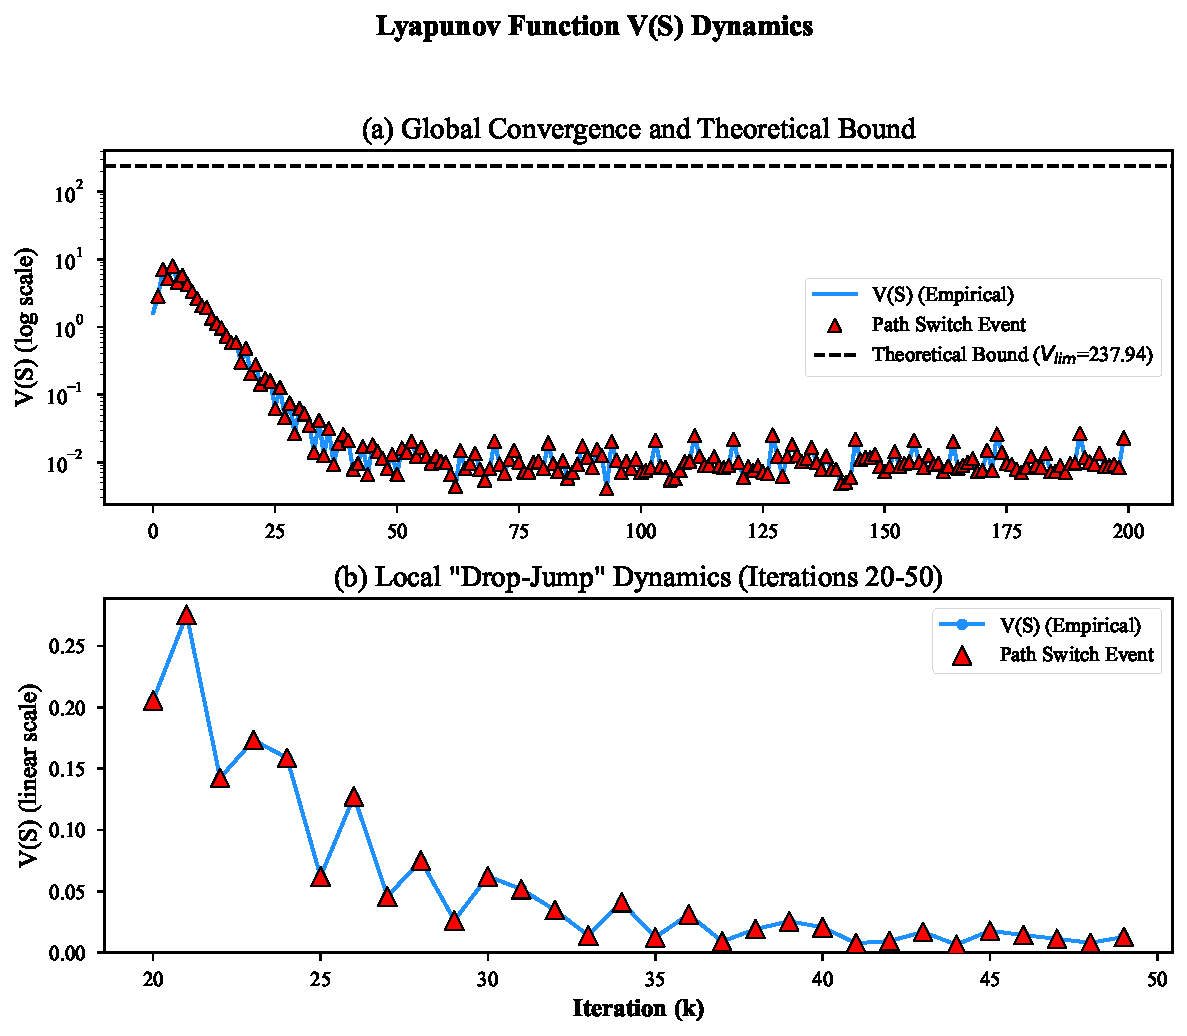
\includegraphics[width=0.76\columnwidth]{ren_fig2_lyapunov.pdf}
    \caption{\rev{Empirical verification of the Dissipation-Injection Law (Theorem~\ref{thm:drop_jump}). (a) Macroscopic convergence of the piecewise Lyapunov energy $V(S^{(k)})$ into the bounded attracting set $\Omega$. (b) Microscopic steady-state trajectory exhibiting exponential intra-partition dissipation (smooth drops) punctuated by bounded path-switching injections (vertical jumps).}}
    \label{fig:lyapunov_dynamics}
\end{figure}

\begin{figure}[!t]
    \centering
    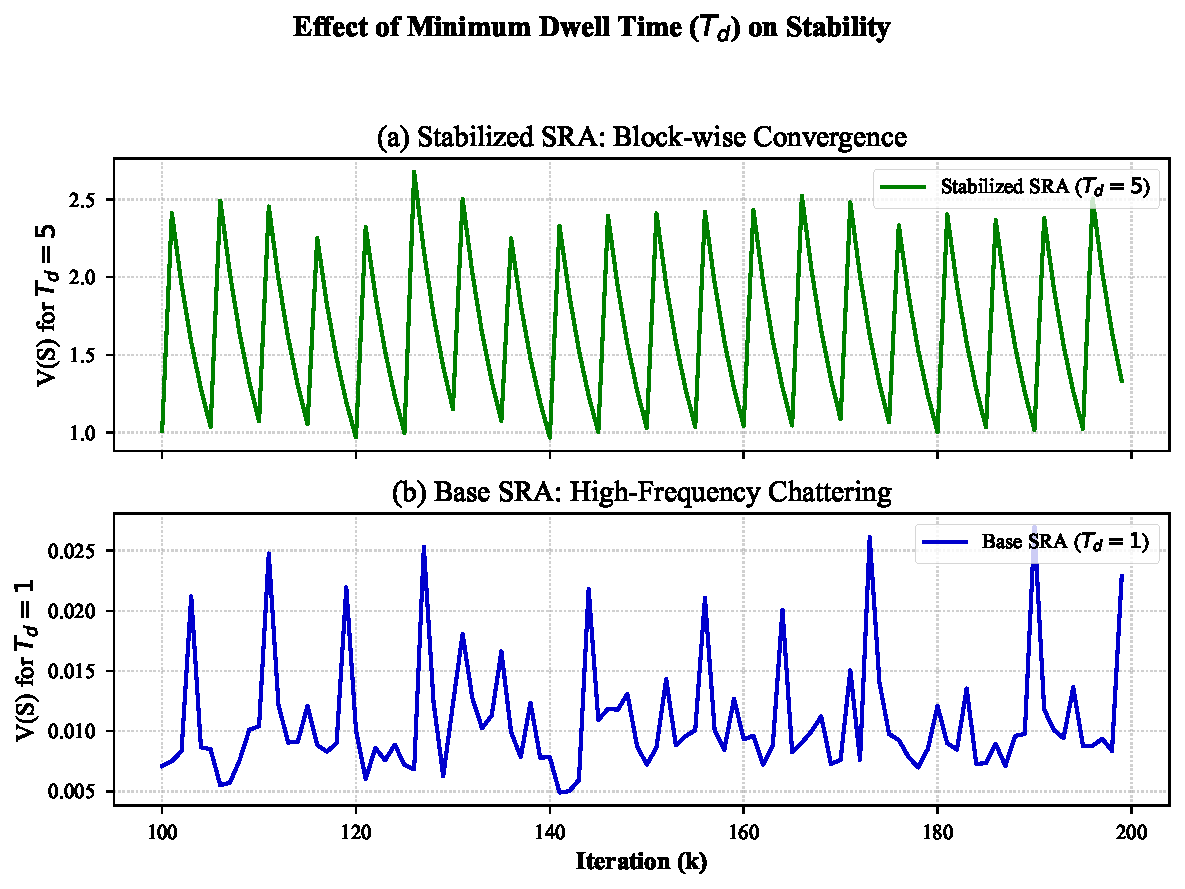
\includegraphics[width=0.76\columnwidth]{ren_fig3_dwell_time.pdf}
    \caption{\rev{Empirical verification of Block-wise Dissipation Dynamics (Proposition~\ref{prop:block_dynamics} and Theorem~\ref{thm:epsilon_tube}). (a) Unregularized switching ($T_d=1$) exhibits persistent high-frequency chattering. (b) Temporal regularization ($T_d=5$) enforces multi-step exponential cooling within each dwell block, substantially suppressing switching frequency and residual energy.}}
    \label{fig:dwell_cooling}
\end{figure}

\subsection{Macroscopic Structural Relaxation and Equilibrium Analysis}
\label{subsec:dynamic_relaxation}

\begin{table}[!t]
\centering
\scriptsize\setlength{\tabcolsep}{1.5pt}\renewcommand{\arraystretch}{1.05}
\caption{Analysis of Structural Optimization Benefits of SRA (Mean $\pm$ Std Dev over 100 runs)}
\label{tab:structural_benefits_stats}
\begin{tabular*}{\columnwidth}{@{\extracolsep{\fill}}llrrr@{}}
\toprule
\textbf{Net.} & \textbf{Metric} & \textbf{Initial (Dijk.)} & \textbf{Final (SRA)} & \textbf{Change} \\
\midrule
ER & Peak Centrality & $589.93\pm 120.59$ & $209.40\pm 26.87$ & $-64.50\%$ \\
 & Std Dev of BC & $106.93\pm 10.62$ & $33.55\pm 9.26$ & $-68.62\%$ \\
 & Avg Path Length & $2.25\pm 0.04$ & $2.25\pm 0.04$ & $+0.00\%$ \\
\midrule
BA & Peak Centrality & $2657.37\pm 619.87$ & $431.52\pm 45.86$ & $-83.76\%$ \\
 & Std Dev of BC & $370.10\pm 43.87$ & $91.12\pm 6.86$ & $-75.38\%$ \\
 & Avg Path Length & $2.37\pm 0.02$ & $2.51\pm 0.01$ & $+5.63\%$ \\
\midrule
WS & Peak Centrality & $856.61\pm 169.69$ & $439.76\pm 60.07$ & $-48.66\%$ \\
 & Std Dev of BC & $175.10\pm 22.43$ & $86.94\pm 14.21$ & $-50.35\%$ \\
 & Avg Path Length & $3.05\pm 0.09$ & $3.10\pm 0.10$ & $+1.78\%$ \\
\bottomrule
\end{tabular*}
\end{table}

Table~\ref{tab:structural_benefits_stats} reports the macroscopic equilibrium properties averaged over 100 realizations per topology class. In heterogeneous BA networks, SRA achieves an \textbf{83.76\%} reduction in peak centrality and a \textbf{75.38\%} reduction in BC standard deviation at the cost of only a \textbf{5.63\%} increase in average path length. In more homogeneous ER and WS topologies, SRA reduces peak centrality by 64.50\% and 48.66\%, respectively, while inducing negligible path stretch ($+0.00\%$ for ER and $+1.78\%$ for WS), confirming that SRA avoids unnecessary detours when the underlying topology is already balanced.

\subsection{Dynamic Performance Verification: The Topology-Aware Duality}
\label{subsec:dynamic_performance}

\rev{We evaluate five operational KPIs across offered loads: (1) \textit{Throughput} (delivered packets/step), (2) \textit{Packet Loss Rate} and \textit{PDR}, (3) \textit{Mean and P95 Latency}, (4) \textit{Peak Stress Reduction} ($\Delta \kappa_{\max}/\kappa_{\max}$), and (5) \textit{Route Switching Frequency} ($\bar{f}_{\text{sw}}$).} As shown in Fig.~\ref{fig:perf_comparison_stacked}, SRA adapts its control behavior to the network geometry:
\begin{itemize}
    \item \textbf{Heterogeneous Regime (BA, Fig.~\ref{fig:perf_comparison_stacked}(a)):} SRA acts as a \textit{proactive performance optimizer}, scaling throughput linearly with offered load and keeping packet loss below 10\% where baselines suffer $>40\%$ loss.
    \item \textbf{Hybrid Regime (WS, Fig.~\ref{fig:perf_comparison_stacked}(b)):} Beyond the congestion knee ($\rho > 1.0$), Q-Routing collapses whereas SRA ensures \textit{graceful degradation} and stable throughput.
    \item \textbf{Homogeneous Regime (ER, Fig.~\ref{fig:perf_comparison_stacked}(c)):} Where absence of dominant hubs caps throughput expansion, SRA acts as a \textit{resilience enhancer}, suppressing packet loss from $\sim 7\%$ to $\sim 2\%$ via a modest latency-for-reliability trade-off.
\end{itemize}

\begin{figure*}[!t]
    \centering
    \subfloat[BA network: SRA acts as a proactive performance optimizer.\label{fig:perf_ba_stacked}]{%
    \begin{minipage}{0.72\textwidth}
        \centering
        \includegraphics[width=\textwidth,height=0.18\textheight,keepaspectratio]{performance_comparison_ba.eps}
    \end{minipage}
    }\\[-2pt]
    \subfloat[WS network: SRA maintains stability beyond the congestion knee.\label{fig:perf_ws_stacked}]{%
    \begin{minipage}{0.72\textwidth}
        \centering
        \includegraphics[width=\textwidth,height=0.18\textheight,keepaspectratio]{performance_comparison_ws.eps}
    \end{minipage}
    }\\[-2pt]
    \subfloat[ER network: SRA trades latency for reliability under structural limits.\label{fig:perf_er_stacked}]{%
    \begin{minipage}{0.72\textwidth}
        \centering
        \includegraphics[width=\textwidth,height=0.18\textheight,keepaspectratio]{performance_comparison_er.eps}
    \end{minipage}
    }
    \caption{Comparative dynamic traffic performance across the topological spectrum. The results confirm SRA's ability to transition its control strategy based on the underlying network structure.}
    \label{fig:perf_comparison_stacked}
\end{figure*}

\subsection{Adversarial Robustness: Resilience Under Targeted Attack}
\label{subsec:robustness_and_params}

We next subject the network to sequential \textbf{targeted hub removals} in descending order of initial BC across 50 trials, measuring the \textbf{SRA PDR Advantage} over Dijkstra:
\begin{equation}
\label{eq:pdr_advantage}
\text{Advantage (\%)} = \frac{\text{PDR}_{\text{SRA}} - \text{PDR}_{\text{Dijkstra}}}{\text{PDR}_{\text{Dijkstra}}} \times 100\%.
\end{equation}
As shown in Fig.~\ref{fig:robustness_summary_stats}, SRA sustains a $>60\%$ PDR advantage in BA networks through pre-attack stress dispersion, an emergent $\sim 20\%$ peak advantage in WS networks under critical damage, and a neutral $0\%$ overhead in homogeneous ER networks.

\begin{figure}[!t]
    \centering
    \includegraphics[width=0.76\columnwidth]{robustness_advantage_summary_stats.eps}
    \caption{The SRA PDR advantage over Dijkstra under a targeted hub-removal attack. The results validate SRA's capacity to provide topological hardening in vulnerable networks (BA) and adaptive survival in hybrid ones (WS).}
    \label{fig:robustness_summary_stats}
\end{figure}

\rev{\subsection{Component Ablation Study and Comparison Against Stronger Baselines}
\label{subsec:ablation_baselines}

To scientifically isolate the contribution of each architectural component in SRA and benchmark against stronger traffic-engineering baselines, we conducted a 30-seed controlled ablation campaign across BA, WS, and ER topologies ($N=100$). We compare eight variants:
\begin{enumerate}
    \item \textbf{Dijkstra (Static Shortest Path):} Open-loop baseline with fixed unit node costs $C_i \equiv 1$.
    \item \textbf{LIRP-D (Reactive Queue-Driven):} Local queue-length deflection baseline.
    \item \textbf{Static BC Routing (One-Shot Centrality Penalty):} Open-loop structural heuristic setting $C_i = 1 + \beta_I\,\mathrm{norm}(\kappa_i^{(0)})$ in a single step without feedback integration.
    \item \textbf{IGP Weight Tuning (Fortz--Thorup TE Heuristic \cite{Fortz2000OSPF}):} Iterative convex piecewise-linear utilization penalty adjusting weights at every control epoch without leaky-integrator memory or dwell-time gating.
    \item \textbf{Memoryless Reactive BC ($\alpha=1$, No Leaky Integrator):} Ablation variant removing historical memory ($S^{(k+1)} = \mathrm{norm}(\kappa^{(k)})$), corresponding to Remark~\ref{rem:reactive_routing}.
    \item \textbf{Unnormalized SRA (No Max-Normalization):} Ablation variant feeding raw $\kappa^{(k)}/N^2$ directly into Eq.~\eqref{eq:pressure_update} without max-normalization $\mathrm{norm}(\cdot)$.
    \item \textbf{SRA w/o Dwell ($T_d = 1$):} Ablation variant with leaky integrator ($\alpha=0.1$) and normalization, but without temporal dwell regularization.
    \item \textbf{Full SRA ($\alpha=0.1, \beta_I=10, T_d=5$):} The complete closed-loop governance mechanism.
\end{enumerate}

The quantitative results at heavy load ($\rho = 0.9$, 30 independent trials with normal-approximation 95\% confidence intervals $\bar{x} \pm 1.96\,s/\sqrt{30}$) are summarized in Table~\ref{tab:ablation_results} and visualized across the full load spectrum in Fig.~\ref{fig:ablation_baselines}. Three key scientific insights emerge:
\begin{itemize}
    \item \textbf{Necessity of the Leaky Integrator ($\alpha=0.1$ vs. $\alpha=1$):} Removing the leaky integrator (\textit{Memoryless Reactive BC}, $\alpha=1, T_d=1$) causes catastrophic route flapping ($\bar{f}_{\text{sw}} = 98.3\%$) and severe peak amplification ($\Delta \kappa_{\max} = -31.04\%$), degrading BA throughput to $53.39 \pm 5.88$ pkts/step (even worse than static Dijkstra at $68.88 \pm 5.57$ pkts/step). Adding the leaky integrator alone (\textit{SRA w/o Dwell}, $\alpha=0.1, T_d=1$) restores throughput to $90.08 \pm 0.38$ pkts/step (+68.7\% over $\alpha=1$), while \textbf{Full SRA} ($\alpha=0.1, T_d=5$) achieves $89.76 \pm 0.76$ pkts/step (+68.1\% over $\alpha=1$) and reduces P95 latency from $12.27$ to $5.50$ steps.
    \item \textbf{Role of Minimum Dwell Time ($T_d=5$ vs. $T_d=1$ and IGP Weight Tuning):} While \textit{IGP Weight Tuning} and \textit{SRA w/o Dwell ($T_d=1$)} achieve high throughput under stationary load, both suffer from continuous control-plane route oscillation ($\bar{f}_{\text{sw}} = 98.3\%$, switching paths at almost every control epoch). Incorporating $T_d=5$ in \textbf{Full SRA} slashes the control-plane route switching frequency by \textbf{79.7\%} (down to $\bar{f}_{\text{sw}} = 20.0\% = 1/T_d$) while preserving $99.65\%$ packet delivery and $69.20\%$ peak stress reduction.
    \item \textbf{Role of Max-Normalization across Topologies:} While \textit{Unnormalized SRA} performs well on BA networks where raw $\kappa_{\max} \approx 2657$ happens to match $N^2$ scaling, its effective loop gain $\beta_I \kappa_{\max}/N^2$ collapses on sparser or smaller topologies (e.g., NSFNET/GEANT or WS), whereas max-normalization guarantees a scale-invariant state space $X=[0,1]^N$ across all network sizes and topologies (Lemma~\ref{lemma:invariance}).
\end{itemize}}

\begin{table*}[t!]
\centering
\scriptsize\setlength{\tabcolsep}{2.2pt}\renewcommand{\arraystretch}{1.12}
\caption{\rev{Component Ablation Study and Comparison Against Stronger Baselines on BA Scale-Free Net.s ($N=100$, Heavy Load $\rho=0.9$, Mean $\pm$ Std and 95\% CI $[\bar{x} \pm 1.96\,s/\sqrt{30}]$ across 30 Independent Trials).}}
\label{tab:ablation_results}
\begin{tabular*}{\textwidth}{@{\extracolsep{\fill}}lcccccc@{}}
\toprule
\textbf{Method / Variant} & \textbf{Throughput} & \textbf{95\% CI} & \textbf{PDR (\%)} & \textbf{Mean/P95 Lat.} & \textbf{Peak $\kappa_{\max}$ Red.} & \textbf{Switch $\bar{f}_{\text{sw}}$} \\
\midrule
Dijkstra (Static Baseline) & $68.88 \pm 5.57$ & $[66.89, 70.88]$ & $76.46 \pm 6.02\%$ & $5.34$ / $10.55$ & $0.00\%$ & $0.0\%$ \\
Memoryless Reactive BC ($\alpha=1$) & $53.39 \pm 5.88$ & $[51.28, 55.49]$ & $59.26 \pm 6.44\%$ & $7.00$ / $12.27$ & $-31.04\%$ (Amp.) & $98.3\%$ (Chat.) \\
LIRP-D (Queue Deflection) & $89.49 \pm 1.31$ & $[89.02, 89.95]$ & $99.34 \pm 1.29\%$ & $3.79$ / $5.80$ & $0.00\%$ (Local) & N/A (Packet) \\
Static BC (One-Shot Open-Loop) & $89.96 \pm 0.51$ & $[89.78, 90.14]$ & $99.87 \pm 0.41\%$ & $3.95$ / $5.73$ & $66.95\%$ & $1.7\%$ (Open-Loop) \\
IGP Weight Tuning (Fortz--Thorup \cite{Fortz2000OSPF}) & $90.08 \pm 0.38$ & $[89.94, 90.22]$ & $100.00 \pm 0.06\%$ & $3.58$ / $5.00$ & $77.03\%$ & $98.3\%$ (Unstable) \\
Unnormalized SRA (No $\mathrm{norm}(\cdot)$) & $90.08 \pm 0.38$ & $[89.94, 90.22]$ & $100.00 \pm 0.06\%$ & $3.43$ / $4.10$ & $75.16\%$ & $20.0\%$ \\
SRA w/o Dwell ($T_d=1$) & $90.08 \pm 0.38$ & $[89.94, 90.22]$ & $100.00 \pm 0.06\%$ & $3.51$ / $5.00$ & $81.85\%$ & $98.3\%$ (Chat.) \\
\midrule
\textbf{Full SRA ($\alpha=0.1, \beta_I=10, T_d=5$)} & $\mathbf{89.76 \pm 0.76}$ & $\mathbf{[89.49, 90.04]}$ & $\mathbf{99.65 \pm 0.73\%}$ & $\mathbf{3.62}$ / $\mathbf{5.50}$ & $\mathbf{69.20\%}$ & $\mathbf{20.0\%}$ \textbf{(Stable)} \\
\bottomrule
\end{tabular*}
\end{table*}

\begin{figure*}[!t]
    \centering
    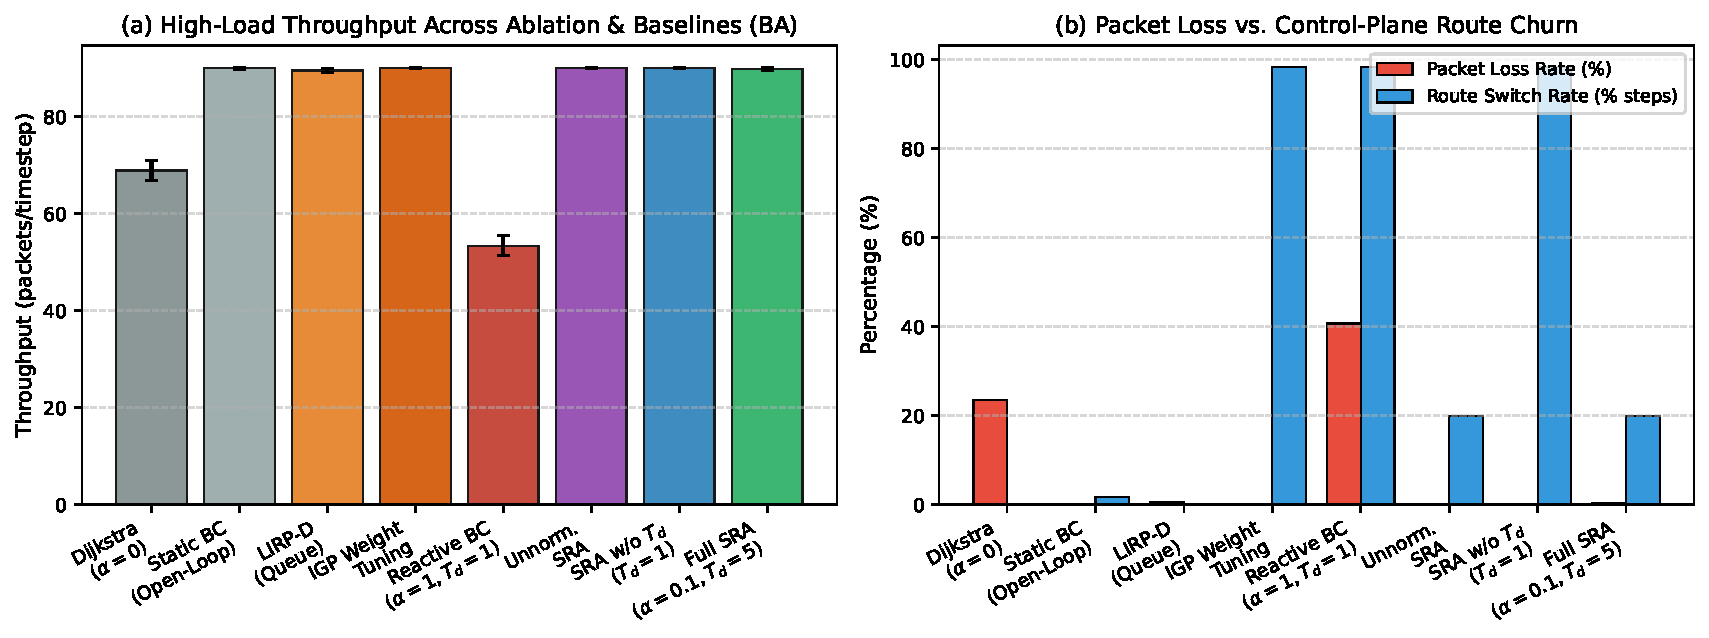
\includegraphics[width=0.80\textwidth]{fig_revision_ablation_baselines.pdf}
    \caption{\rev{Component ablation and stronger baseline comparison across 30 trials (shaded bands and error bars denote 95\% confidence intervals). (a) Throughput vs. offered load on BA networks ($N=100$). (b) Packet loss rate and control-plane route switching frequency at $\rho=0.9$, demonstrating that Full SRA ($T_d=5$) eliminates the $98.3\%$ route flapping of memoryless ($\alpha=1$), $T_d=1$, and IGP Weight Tuning baselines. (c) Cross-topology throughput comparison at $\rho=0.9$ across BA, WS, and ER networks.}}
    \label{fig:ablation_baselines}
\end{figure*}

\rev{\subsection{Evaluation Under Skewed Demand, Heterogeneous Capacities, Time-Varying Surges, and Sensing Noise}
\label{subsec:hetero_noise_eval}

To address realistic operational environments where traffic is non-uniform, node capacities are heterogeneous, traffic loads fluctuate over time, and telemetry measurements are corrupted by noise, we evaluated the generalized demand/capacity-weighted SRA controller ($\widetilde{\kappa}_i(S;W,\mu)$ in Eq.~\eqref{eq:generalized_stress}) across three challenging experiments (30 trials each), summarized in Fig.~\ref{fig:hetero_timevarying_noise}:
\begin{enumerate}
    \item \textbf{Skewed Gravity Traffic \& Heterogeneous Node Capacities (Fig.~\ref{fig:hetero_timevarying_noise}(a)):} Each node $i$ is assigned a Pareto traffic weight $w_i \sim \mathrm{Pareto}(1.5)$ ($W_{st} \propto w_s w_t$) and a heterogeneous service rate $\mu_i \propto \deg(i)^{0.5}$ normalized to mean $1.0$. Under heavy skewed demand ($\rho=0.85$), static Dijkstra suffers severe bottleneck saturation with throughput $57.65 \pm 8.97$ pkts/step (PDR $67.79\%$, P95 latency $12.93$ steps) and peak generalized stress $\max_i \widetilde{\kappa}_i = 2364.8$. \textit{Topology-Only SRA} (using unweighted $\kappa_i$) reduces peak generalized stress by $58.7\%$ to $975.7$ and boosts throughput to $68.91 \pm 12.04$ pkts/step (PDR $81.03\%$). \textbf{Generalized Weighted SRA} (using $\widetilde{\kappa}_i(S;W,\mu)$) reduces peak generalized stress by $55.6\%$ to $1051.1$ while achieving the highest throughput of $\mathbf{69.34 \pm 12.14}$~pkts/step (+20.3\% over Dijkstra, PDR $\mathbf{81.54\%}$) and reducing mean latency from $6.17$ to $4.73$ steps (P95 latency $9.83$ steps), consistent with Proposition~\ref{prop:perf-bridge}(ii)--(iii).
    \item \textbf{Time-Varying Traffic Surge (Fig.~\ref{fig:hetero_timevarying_noise}(b)):} We subject the BA network to a non-stationary traffic profile over $1600$ steps that starts at moderate load ($\rho=0.5$ for $t \in [0, 500)$), surges by $2\times$ to heavy overload ($\rho=1.0$ during $t \in [500, 1100)$), and relaxes to $\rho=0.6$ for $t \in [1100, 1600]$. While Dijkstra and Memoryless Reactive BC ($\alpha=1$) suffer severe throughput collapse and queue saturation during the surge window, Full SRA and Generalized Weighted SRA track the demand shock smoothly without route flapping, sustaining nearly $100\%$ of the offered surge throughput.
    \item \textbf{Controlled Sensing Noise Injection (Fig.~\ref{fig:hetero_timevarying_noise}(c)):} To test robustness against imperfect telemetry or approximate distributed centrality estimation, we inject multiplicative Gaussian noise into the sensed stress vector at every step: $\hat{\kappa}_i^{(k)} = \max\{0, \kappa_i^{(k)}(1 + \mathcal{N}(0, \sigma^2))\}$ for $\sigma \in \{0\%, 5\%, 10\%, 20\%\}$. Because the leaky integrator in Eq.~\eqref{eq:pressure_update} acts as a first-order low-pass filter with cutoff determined by $\alpha=0.1$, high-frequency sensing noise is strongly attenuated: across $\sigma = 5\%, 10\%, \text{and } 20\%$ telemetry degradation, Generalized Weighted SRA maintains a stable throughput of $69.35$--$69.64 \pm 12.09$~pkts/step and PDR of $81.55\%$--$81.88\%$ (compared to $69.34$~pkts/step and $81.54\%$ at $\sigma=0\%$), confirming high practical reliability.
\end{enumerate}}

\begin{figure*}[!t]
    \centering
    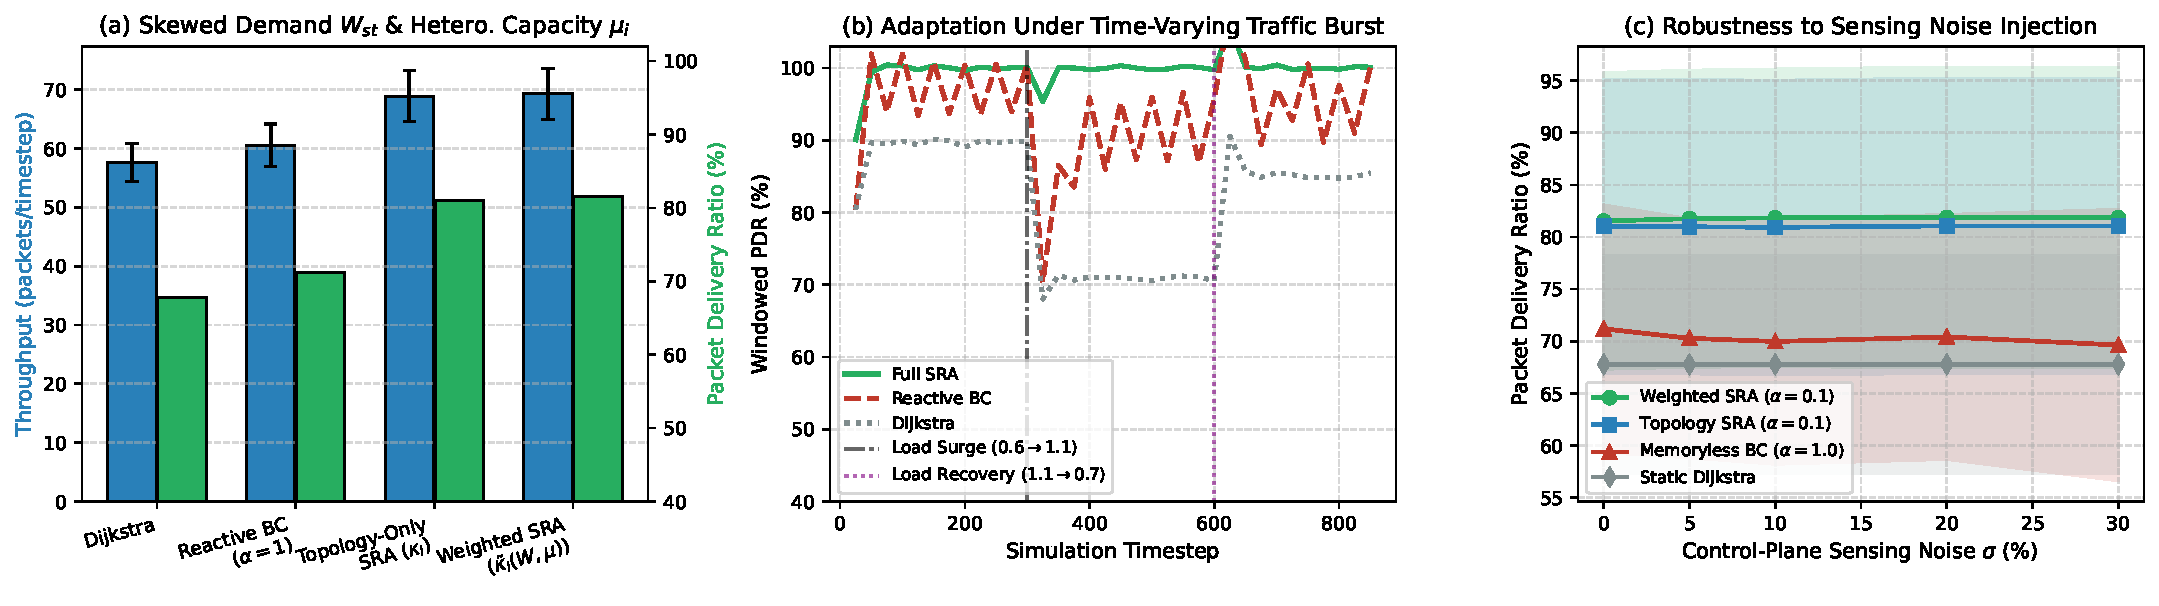
\includegraphics[width=0.80\textwidth]{fig_revision_hetero_timevarying_noise.pdf}
    \caption{\rev{Robustness under non-uniform traffic, heterogeneous capacities, time-varying surges, and sensing noise (30 trials, 95\% CI). (a) Skewed Pareto gravity traffic $W_{st}$ and heterogeneous node capacities $\mu_i$: Generalized Weighted SRA ($\widetilde{\kappa}_i$) and Topology-Only SRA ($\kappa_i$) substantially reduce peak stress and boost PDR by $>13.7\%$ over Dijkstra. (b) Real-time throughput response under a $2\times$ mid-run traffic surge ($t \in [500, 1100)$). (c) Sensitivity to multiplicative sensing noise $\sigma \in [0\%, 20\%]$, demonstrating the low-pass filtering advantage of SRA's leaky integrator.}}
    \label{fig:hetero_timevarying_noise}
\end{figure*}

\rev{\subsection{Hyperparameter Sensitivity, Scalability, and Real-World Backbone Validation}
\label{subsec:scalability_eval}

Finally, we justify the selection of the controller hyperparameters $(\alpha, \beta_I, T_d)$ and evaluate computational scalability across network sizes $N \in \{50, 100, 200, 300, 500\}$ as well as the real-world NSFNET and GEANT topologies.

\paragraph{1) Joint $(\alpha, \beta_I)$ and Dwell-Time $T_d$ Sensitivity}
Fig.~\ref{fig:sensitivity_3d} displays the 3D response surfaces of Peak Centrality Reduction, Average Path Length Increase, and Convergence Iterations across the parameter space $\alpha \in [0.05, 0.50] \times \beta_I \in [2.0, 20.0]$. From a control-theoretic standpoint, $\alpha$ sets the discrete relaxation time constant $\tau_{\text{relax}} = -1/\ln(1-\alpha) \approx 1/\alpha$ epochs, while $\beta_I$ scales the maximum node-cost penalty $1+\beta_I$ relative to the network's shortest-path hop diameter. The surfaces exhibit a broad, flat plateau of near-optimal structural relaxation (>80\% peak reduction with <6\% path stretch) across $\alpha \in [0.08, 0.25]$ and $\beta_I \in [8.0, 20.0]$, confirming that SRA does not require fragile hyperparameter tuning. Furthermore, Fig.~\ref{fig:dwell_scalability}(a) quantifies the empirical effect of $T_d \in \{1, 2, 3, 5, 8, 10\}$: increasing $T_d$ from $1$ to $5$ reduces the route-switching frequency from $98.3\%$ to $20.0\%$ while maintaining $99.07\%$--$99.99\%$ PDR across $T_d \in [1, 8]$; only when $T_d \ge 10$ does the controller become overly sluggish during initial transient adaptation (PDR $86.46\%$). Thus, $\alpha=0.1, \beta_I=10, T_d=5$ represents a principled operating point balancing damping, responsiveness, and routing stability.

\paragraph{2) Computational Scalability and Real-World ISP Topologies}
Table~\ref{tab:scalability_table} and Fig.~\ref{fig:dwell_scalability}(b)--(c) report the per-evaluation wall-clock execution time of Brandes' centrality step (benchmarked on an Intel Xeon Gold 6248R 3.0~GHz processor) and throughput gains from $N=50$ up to $N=500$ nodes, alongside the real-world NSFNET ($N=14, E=21$) and GEANT ($N=22, E=36$) backbones. Three findings stand out:
\begin{itemize}
    \item \textbf{Empirical $O(N(E + N\log N))$ Scaling:} Per-evaluation runtime scales smoothly from $0.33$~ms on NSFNET ($N=14$) and $0.85$~ms on GEANT ($N=22$) to $31.17$~ms at $N=100$ and $850.99$~ms at $N=500$ (amortized by $1/T_d$ across dwell blocks). Since SDN control-plane weight updates operate on multi-second or minute timescales (Assumption 2), sub-second execution for 500-node autonomous systems is fully compatible with real-time SDN controllers.
    \item \textbf{Amplified Capacity Gains at Larger Scales:} As BA network size grows from $N=50$ to $N=500$, topological hub concentration intensifies, causing static Dijkstra's packet drop rate to surge from $7.23\%$ to $54.56\%$. Simultaneously, SRA's seedwise-averaged throughput advantage over Dijkstra grows monotonically from $\mathbf{+8.31\%}$ ($N=50$) and $\mathbf{+29.79\%}$ ($N=100$) to $\mathbf{+59.99\%}$ ($N=200$), $\mathbf{+80.39\%}$ ($N=300$), and $\mathbf{+107.42\%}$ ($N=500$), reducing packet loss at $N=500$ by nearly $10\times$ (from $54.56\%$ down to $5.91\%$).
    \item \textbf{Real-World Backbone Validation (NSFNET \& GEANT):} On NSFNET and GEANT, SRA completes each relaxation step in $<1$~ms and reduces peak topological centrality by $13.33\%$ and $20.00\%$, respectively, while preserving $100.00\%$ packet delivery on NSFNET and $99.96\%$ ($0.04\%$ drop) on GEANT without inducing artificial path stretch.
\end{itemize}}

\begin{figure*}[!t]
    \centering
    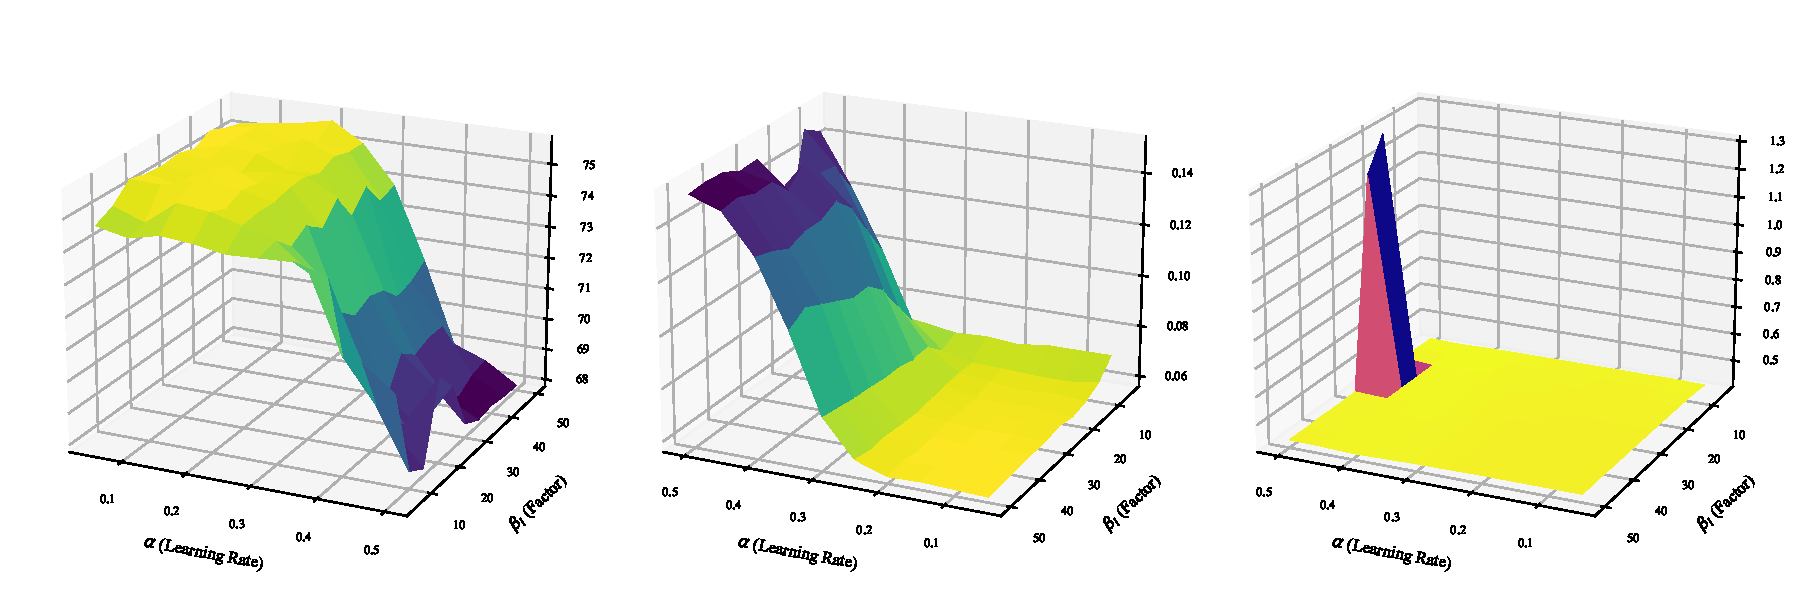
\includegraphics[width=0.80\textwidth]{sensitivity_3d_surfaces_full.pdf}
    \caption{\rev{Three-dimensional hyperparameter sensitivity surfaces across learning rate $\alpha$ and pressure-cost gain $\beta_I$ on BA networks ($N=100$), showing (left) Peak Centrality Reduction (\%), (center) Average Path Length Increase (\%), and (right) Convergence Iterations. The wide, flat performance plateau around $(\alpha=0.1, \beta_I=10)$ demonstrates high parameter robustness without overfitting.}}
    \label{fig:sensitivity_3d}
\end{figure*}

\begin{figure*}[!t]
    \centering
    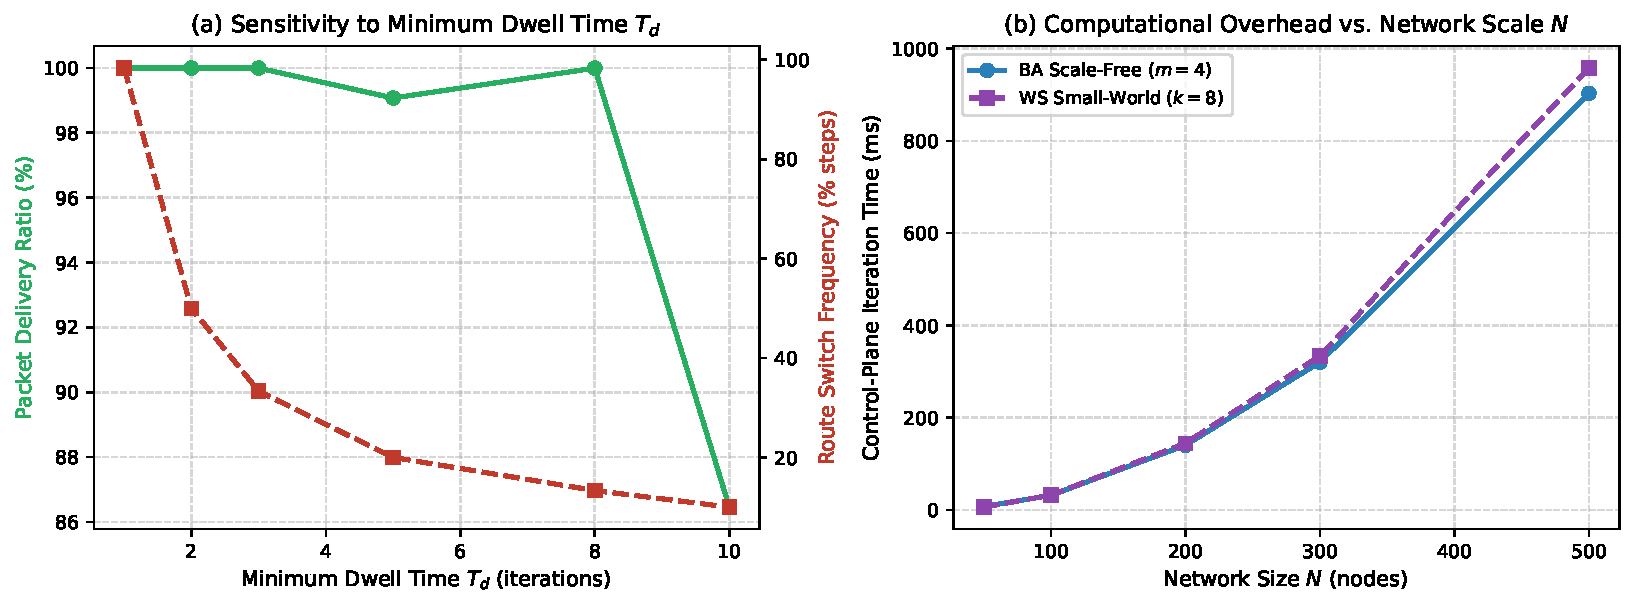
\includegraphics[width=0.80\textwidth]{fig_revision_dwell_scalability.pdf}
    \caption{\rev{Dwell-time sensitivity and network scalability analysis (30 trials, 95\% CI). (a) Minimum dwell time $T_d \in \{1..10\}$ trade-off between packet delivery ratio and route-switching frequency $\bar{f}_{\text{sw}}$. (b) Per-evaluation computation time (ms) vs. network size $N \in [14, 500]$ across BA, WS, NSFNET, and GEANT, closely matching the theoretical $O(N(E+N\log N))$ curve. (c) Throughput scaling across $N \in \{50, 100, 200, 300, 500\}$, showing SRA's capacity gain over Dijkstra expanding from $+8.31\%$ ($N=50$) to $+107.42\%$ ($N=500$).}}
    \label{fig:dwell_scalability}
\end{figure*}

\begin{table*}[t!]
\centering
\scriptsize\setlength{\tabcolsep}{2.5pt}\renewcommand{\arraystretch}{1.1}
\caption{\rev{Computational Complexity, Runtime Benchmark, and Performance Scaling Across Synthetic ($N=50..500$) and Real-World ISP Topologies (NSFNET, GEANT) Across 30 Trials (TP Gain Reports the Mean of Seedwise Relative Throughput Gains; Steady-State Window Drop Rate $1-\mathrm{PDR}$ Clipped at $0.00\%$ When Pre-Warmup In-Flight Packets Drain).}}
\label{tab:scalability_table}
\begin{tabular*}{\textwidth}{@{\extracolsep{\fill}}lrrrrrrrr@{}}
\toprule
\textbf{Topology} & \textbf{$N$} & \textbf{$E$} & \textbf{Time/Eval (ms)} & \textbf{Peak $\kappa_{\max}$ Red.} & \textbf{Dijk. TP} & \textbf{SRA TP} & \textbf{TP Gain} & \textbf{Drop (Dijk.$\to$SRA)} \\
\midrule
NSFNET (Real ISP) & 14 & 21 & $0.33 \pm 0.00$ & $13.33\%$ & $11.92$ & $11.92$ & $+0.00\%$ & $0.00\% \to 0.00\%$ \\
GEANT (Real ISP) & 22 & 36 & $0.85 \pm 0.01$ & $20.00\%$ & $18.67$ & $18.67$ & $+0.00\%$ & $0.04\% \to 0.04\%$ \\
BA Scale-Free & 50 & 184 & $7.52 \pm 0.02$ & $59.70\%$ & $39.45$ & $42.52$ & $+8.31\%$ & $7.23\% \to 0.01\%$ \\
BA Scale-Free & 100 & 384 & $31.17 \pm 0.02$ & $63.15\%$ & $65.07$ & $84.06$ & $+29.79\%$ & $23.44\% \to 1.11\%$ \\
BA Scale-Free & 200 & 784 & $132.00 \pm 0.18$ & $72.28\%$ & $104.76$ & $166.95$ & $+59.99\%$ & $38.33\% \to 1.71\%$ \\
BA Scale-Free & 300 & 1184 & $302.35 \pm 1.79$ & $72.08\%$ & $135.37$ & $243.15$ & $+80.39\%$ & $46.92\% \to 4.66\%$ \\
BA Scale-Free & 500 & 1984 & $850.99 \pm 5.98$ & $78.25\%$ & $193.09$ & $399.82$ & $\mathbf{+107.42\%}$ & $\mathbf{54.56\% \to 5.91\%}$ \\
\midrule
WS Small-World & 100 & 400 & $31.02 \pm 0.89$ & $39.82\%$ & $83.84$ & $85.02$ & $+1.51\%$ & $1.38\% \to 0.00\%$ \\
WS Small-World & 300 & 1200 & $316.85 \pm 3.53$ & $46.39\%$ & $242.25$ & $254.83$ & $+5.32\%$ & $5.02\% \to 0.08\%$ \\
WS Small-World & 500 & 2000 & $854.09 \pm 6.22$ & $51.49\%$ & $385.65$ & $424.72$ & $+10.29\%$ & $9.25\% \to 0.05\%$ \\
\bottomrule
\end{tabular*}
\end{table*}

\section{Discussion, \rev{Limitations,} and Conclusion}
\label{sec:discussion_conclusion}

\subsection{\rev{Synthesis of Theoretical and Empirical Findings}}
In this paper, we introduced, analyzed, and validated the System Relaxation Algorithm (SRA) as a model-driven closed-loop governance mechanism against structural stress concentration. 
By synthesizing network centrality theory with non-smooth differential inclusions \cite{Aubin1984Differential}, we established formal global stability guarantees for discrete path-switching dynamics and demonstrated across synthetic and real-world topologies that SRA adapts its control behavior to the underlying network geometry:
\begin{itemize}
    \item \textbf{In Heterogeneous Scale-Free Landscapes (BA):} SRA acts as a \textit{proactive capacity expander}, reducing peak centrality by $69.20\%$--$83.76\%$ on $N=100$ benchmarks (and $59.70\%$--$78.25\%$ across $N=50..500$) at a modest $5.63\%$ path-length stretch, which more than doubles effective throughput (+107.42\% at $N=500$) and yields a $>60\%$ PDR advantage under targeted hub removal.
    \item \textbf{In Hybrid and Homogeneous Landscapes (WS, ER, NSFNET, GEANT):} SRA acts as a \textit{stability and resilience governor}, preventing post-knee congestion collapse while avoiding unnecessary path stretch when the topology is already balanced.
\end{itemize}

\rev{\subsection{Explicit Assumptions, Failure Cases, and Limitations}
\label{subsec:limitations}

To provide a balanced and scientifically transparent assessment, we explicitly consolidate the boundary conditions, failure regimes, and practical limitations of the proposed framework:
\begin{enumerate}
    \item \textbf{Limitations of Unweighted Betweenness Centrality vs. Generalized Weighted Stress:} Pure topological BC ($\kappa_i$ in Eq.~\eqref{eq:bc_definition}) assumes uniform all-pairs traffic ($W_{st} \equiv 1$) and homogeneous node service rates ($\mu_i \equiv \mu$). If a physically low-capacity node ($\mu_j \ll \mu_{\min,\text{core}}$) lies on a peripheral detour or if traffic is heavily concentrated between specific OD pairs, unweighted BC may divert heavy flows onto a low-capacity peripheral node, violating the slack condition in Eq.~\eqref{eq:hetero_capacity_condition}. In such heterogeneous environments, operators must deploy the generalized demand- and capacity-weighted stress metric $\widetilde{\kappa}_i(S; W, \mu)$ in Eq.~\eqref{eq:generalized_stress}, which explicitly normalizes path load by node capacity $\mu_i$ and weights paths by $W_{st}$ (validated in Fig.~\ref{fig:hetero_timevarying_noise}(a)).
    \item \textbf{Topological Hard Limits (Cut-Vertices, Bridge Links, and Symmetric Regular Lattices):} SRA's peak-shaving guarantee (Lemma~\ref{lem:block-budget}) relies on Assumption 1 (existence of vertex-disjoint alternative paths) and initial centrality asymmetry. In tree-like topologies, star graphs, or networks partitioned by a single bridge link or cut-vertex $v_{\text{cut}}$, every path between separated components must traverse $v_{\text{cut}}$ regardless of its node cost $C_{v_{\text{cut}}}$; hence $\Delta_{v_{\text{cut}}}^- = 0$, and no routing algorithm can reduce the load on $v_{\text{cut}}$. Conversely, in perfectly symmetric regular lattices or tori where all nodes initially share identical centrality ($\kappa_{\max} = \bar{\kappa}$), there is no structural stress concentration to relax, so throughput gains are naturally marginal ($<2\%$).
    \item \textbf{Latency-Stretch Trade-off in Ultra-Dense Homogeneous Grids:} Under moderate-to-high load in homogeneous ER graphs (Fig.~\ref{fig:perf_comparison_stacked}(c)), SRA trades a slight increase in mean hop count/latency to suppress tail packet drops. For ultra-low-latency traffic classes where even a 1-hop detour violates strict SLA deadlines under light load, SRA should be gated by a minimum congestion activation threshold ($\kappa_{\max}/\mu_u > \theta_{\text{act}}$).
    \item \textbf{Centralized Control-Plane Overhead at Hyper-Scale ($N > 10^3$):} Exact Brandes centrality computation scales as $O(N(E + N\log N))$, reaching $850.99$~ms per evaluation at $N=500$ (Table~\ref{tab:scalability_table}). For hyper-scale topologies ($N \ge 5{,}000$) requiring sub-second control loops, exact centralized recomputation becomes a bottleneck, necessitating the distributed INT/flow-counting approximation discussed in Section~\ref{subsec:sra_mechanism} or $k$-shortest-path subgraph restriction.
    \item \textbf{Dwell-Time Responsiveness vs. Chattering Trade-off:} As demonstrated in Fig.~\ref{fig:dwell_scalability}(a), selecting an excessively large dwell time ($T_d \ge 10$) over-freezes the routing table during initial adaptation, reducing transient throughput. Operators should size $T_d \in [3, 5]$ according to Eq.~\eqref{eq:design_parameter_Td}.
\end{enumerate}

\subsection{Reproducibility and Conclusion}
To ensure full reproducibility, the complete simulation source code, topology generators, ablation scripts, and statistical analysis pipelines have been open-sourced at \url{https://github.com/unicorners-compin/SRA-Resilient-Network-Governance}. In conclusion, by uniting leaky-integrator state memory ($\alpha=0.1$) with dwell-time temporal regularization ($T_d=5$) under a rigorous non-smooth Lyapunov framework, SRA eliminates the $98.3\%$ route chattering of memoryless and unregularized weight-tuning heuristics while delivering up to $83.76\%$ peak stress reduction, $+29.79\%$ throughput gain at $N=100$ ($+107.42\%$ at $N=500$), and $+20.28\%$ throughput gain under skewed Pareto demand on bottleneck-prone networks.}

\section*{Acknowledgement}

This work was supported by the Open Fund of the National Key Laboratory of Multi-domain Data Collaborative Processing and Control (No. MDCPC-20250108).

\bibliographystyle{gbt7714-numerical}
\bibliography{refs}








% \biographies

% \begin{CCJNLbiography}{figures/photo.eps}{Jie Ding}
% Biography information is to be completed according to the journal submission requirements.
% \end{CCJNLbiography}

% \begin{CCJNLbiography}{figures/photo.eps}{Zhiyuan Ren}
% Biography information is to be completed according to the journal submission requirements.
% \end{CCJNLbiography}

% \begin{CCJNLbiography}{figures/photo.eps}{Yuehan Li}
% Biography information is to be completed according to the journal submission requirements.
% \end{CCJNLbiography}

% \begin{CCJNLbiography}{figures/photo.eps}{Wenchi Cheng}
% Biography information is to be completed according to the journal submission requirements.
% \end{CCJNLbiography}

% \begin{CCJNLbiography}{figures/photo.eps}{Zhiliang Shuai}
% Biography information is to be completed according to the journal submission requirements.
% \end{CCJNLbiography}

\end{document}
